\documentclass[10pt,letterpaper]{article}
\usepackage[margin=.9in]{geometry}
\usepackage{amsmath,amssymb,graphicx,booktabs,hyperref}
\hypersetup{hidelinks,pdftitle={Numerical investigations of three-dimensional cubic dispersion and weighted decay},pdfauthor={}}
\numberwithin{equation}{section}
\newtheorem{proposition}{Proposition}[section]
\newtheorem{definition}[proposition]{Definition}
\newcommand{\norm}[1]{\left\|#1\right\|}
\newcommand{\takeaway}[1]{\par\medskip\noindent\textbf{Remark.} #1\par\medskip}
\newcommand{\callout}[1]{\par\medskip\noindent #1\par\medskip}
\DeclareFontShape{OT1}{cmr}{m}{n}{<->cmr10}{}
\DeclareMathSizes{8}{10}{7}{7}\DeclareMathSizes{12}{12}{7}{7}
\DeclareMathSizes{9}{10}{7}{7}\DeclareMathSizes{10}{10}{7}{7}
\DeclareFontShape{OT1}{cmr}{bx}{n}{<->cmbx10}{}
\DeclareFontShape{TU}{lmr}{m}{n}{<->\UnicodeFontFile{lmroman10-regular}{\UnicodeFontTeXLigatures}}{}
\DeclareFontShape{TU}{lmr}{bx}{n}{<->\UnicodeFontFile{lmroman10-bold}{\UnicodeFontTeXLigatures}}{}
\DeclareFontShape{TU}{lmr}{m}{it}{<->\UnicodeFontFile{lmroman10-italic}{\UnicodeFontTeXLigatures}}{}
\setlength{\parindent}{1.2em}
\setlength{\parskip}{3pt}
\setlength{\emergencystretch}{1.5em}
\renewcommand{\topfraction}{.9}\renewcommand{\bottomfraction}{.8}
\renewcommand{\textfraction}{.08}\renewcommand{\floatpagefraction}{.65}
\newcommand{\MassError}{$1.11\times10^{-16}$}
\newcommand{\SymmetryError}{$1.76\times10^{-16}$}
\newcommand{\PlaneError}{$2.18\times10^{-15}$}
\newcommand{\ReverseError}{$6.69\times10^{-16}$}
\newcommand{\QuadError}{$3.91\times10^{-9}$}
\newcommand{\PeakPercent}{0.556}
\newcommand{\Runtime}{12.4}
\newcommand{\FinalRows}{$1$ & unshifted & 0.473 & 3.598 & 3.598 & 3.866 \\
$1$ & x shift & 0.438 & 3.891 & 3.598 & 4.140 \\
$1$ & z shift & 0.414 & 4.849 & 4.849 & 3.090 \\
$-1/3$ & unshifted & 0.481 & 3.598 & 3.598 & 3.629 \\
$-1/3$ & x shift & 0.444 & 3.891 & 3.598 & 3.919 \\
$-1/3$ & z shift & 0.303 & 4.849 & 4.849 & 4.872 \\
$0$ & unshifted & 0.467 & 3.598 & 3.598 & 3.598 \\
$0$ & x shift & 0.433 & 3.891 & 3.598 & 3.891 \\
$0$ & z shift & 0.346 & 4.849 & 4.849 & 3.598 \\}
\newcommand{\GridRows}{$32^3$ & $1.89\times10^{-1}$ & $2.05\times10^{-1}$ & $1.68\times10^{-1}$ \\
$64^3$ & $7.75\times10^{-6}$ & $8.24\times10^{-6}$ & $7.38\times10^{-6}$ \\
$96^3$ & $2.13\times10^{-14}$ & $2.15\times10^{-14}$ & $1.90\times10^{-14}$ \\}
\newcommand{\DomainRows}{$1$ & $5.87\times10^{-3}$ & $2.00\times10^{-5}$ & $2.07\times10^{-4}$ \\
$-1/3$ & $3.70\times10^{-2}$ & $1.71\times10^{-5}$ & $1.55\times10^{-5}$ \\
$0$ & $3.95\times10^{-3}$ & $1.49\times10^{-7}$ & $5.58\times10^{-7}$ \\}
\newcommand{\RefinedRows}{Homogeneous & Gaussian & 0.00731 & 1.11\% & 0.18\% \\
Homogeneous & Compact bump & 0.00677 & 0.43\% & 0.03\% \\
Homogeneous & Near degeneracy & 0.00499 & 1.62\% & 0.24\% \\
Homogeneous & Random (33) & 0.00618 & 1.61\% & 0.29\% \\
Inhomogeneous & Gaussian & 0.00468 & 0.01\% & 0.05\% \\
Inhomogeneous & Compact bump & 0.00431 & 0.00\% & 0.54\% \\
Inhomogeneous & Near degeneracy & 0.00344 & 1.36\% & 0.01\% \\
Inhomogeneous & Random (33) & 0.00415 & 0.00\% & 0.04\% \\}
\newcommand{\ObservedResult}{The inhomogeneous Gaussian and random packet ratios begin to flatten: from $t=8$ to $16$ they grow by 3.42\% and 0.78\%, respectively. The near-degeneracy ratios continue to rise more visibly, as do several homogeneous cases. This suggests different transient time scales; it does not establish their eventual behavior.}
\newcommand{\CheckResult}{Across all 24 checked case--time combinations, the largest peak changes are 1.62\% under domain enlargement and 0.94\% under grid refinement. All pass the exploratory 2\% screen.}
\newcommand{\LongRows}{Homogeneous & Gaussian & 0.00917 & 0.00999 & 1.043 \\
Homogeneous & Near degeneracy & 0.00833 & 0.00888 & 1.074 \\
Inhomogeneous & Gaussian & 0.00407 & 0.00372 & 1.293 \\
Inhomogeneous & Near degeneracy & 0.00558 & 0.00586 & 1.096 \\}
\newcommand{\LongDomain}{0.141\%}
\newcommand{\LongQuad}{0.020\%}
\newcommand{\LongEdge}{0.586\%}

\newcommand{\SelectedRows}{Random seed 33 & 0.003767 & 0.001491 & 60.4\% & 0.005556 \\
Two packets & 0.001433 & 0.000844 & 41.1\% & 0.003667 \\}
\newcommand{\ResearchScaleError}{4.4e-16}
\newcommand{\ResearchPass}{70}
\newcommand{\ResearchFollowPass}{8}
\newcommand{\ResearchFollowChange}{0.0011\%}
\newcommand{\ResearchCorrection}{2.288\%}
\newcommand{\ResearchQuadError}{4.4e-12}
\newcommand{\ResearchQuadTail}{7.5e-12}
\newcommand{\SpatialRows}{Homogeneous & Gaussian & 0.0130\% & 0.0000\% & 0.0046\% & 0.0025\% \\
Homogeneous & Near degeneracy & 0.0020\% & 0.0000\% & 0.0007\% & 0.0003\% \\
Inhomogeneous & Gaussian & 0.0001\% & 0.0000\% & 0.0000\% & 0.0000\% \\
Inhomogeneous & Near degeneracy & 0.0033\% & 0.0000\% & 0.0026\% & 0.0004\% \\}
\newcommand{\SpatialLocations}{Homogeneous & Gaussian & 0.0099887 & -20.7469 & 0.0000 & 0.00000 \\
Homogeneous & Near degeneracy & 0.0088803 & 7.7961 & 6.5381 & 0.00079 \\
Inhomogeneous & Gaussian & 0.0037238 & -8.9154 & 0.0000 & 0.00002 \\
Inhomogeneous & Near degeneracy & 0.0058621 & -841.2464 & 0.0000 & 0.00021 \\}
\newcommand{\SpatialLocationDrift}{0.00079}
\newcommand{\SpatialPeakDrift}{0.00459\%}
\newcommand{\SpatialQuadTighten}{$3.67\times10^{-12}\%$}
\newcommand{\SpatialBoundary}{0.00516\%}
\newcommand{\SpatialPassed}{4}

\title{Numerical Investigations of Three-Dimensional\\Cubic Dispersion and Weighted Decay}
\author{}
\date{Research checkpoint: September 10, 2026}
\begin{document}
\maketitle
\begin{abstract}
We document numerical experiments for linear three-dimensional cubic propagators
arising in the Dysthe research context. The principal observable is the normalized
weighted peak $t^{7/6}\|\,|D_x+\beta|^{1/2}S(t)f\|_\infty/\|f\|_1$.
The study combines Fourier propagation for varied artificial initial data with
Gaussian-specific transverse integration, spatial refinement, and independent
oscillatory quadrature. Four Gaussian-based decay curves are computed through
$t=256$, where all four candidate maxima pass a 0.1\% spatial stability screen.
Additional experiments examine cubic scaling, spectral location, cancellation
and concentration. Three-dimensional level surfaces and planar slices illustrate
selected random and two-packet solutions. The computations establish numerical
consistency within the tested settings; they establish neither a new uniform
upper bound nor a counterexample. A scaling argument explains why an improved
homogeneous exponent requires a modified input class or right-hand-side norm.
\end{abstract}
\noindent\textbf{Keywords:} cubic dispersion; Dysthe equation; weighted decay;
Fourier methods; oscillatory integrals; numerical convergence.
\tableofcontents
\clearpage

\section{Introduction and research objective}

\subsection{Scope and principal findings}\label{summary}
We have developed a numerical workflow for linear cubic dispersion in three
independent spatial coordinates, with a visual explanation of wave envelopes and
an explicit connection to the weighted estimate in the supplied manuscript.
The workflow separates finite-box FFT experiments from Gaussian-specific
whole-space transverse integration.

\textbf{1. The observable matters.} Ordinary envelope peaks describe visible
spreading. The estimate instead controls a fractionally weighted solution. At
$\alpha=1/2$ and $p=\infty$, the diagnostic is
\begin{equation}
 R(t;f)=t^{7/6}\big\||D_x+\beta|^{1/2}S(t)f\big\|_\infty/\|f\|_1.
\end{equation}
A rising ratio on a finite interval is compatible with a bounded estimate; the
manuscript does not specify a numerical failure threshold.

\textbf{2. The most reliable long-time evidence is spatial.} For four
Gaussian-based cases at $256$, two longitudinal enlargements and an independent
radial extension pass the 0.1\% screen. The largest final change in locally
refined peak magnitude is 0.00459\%, and peak-location drift is below 0.0008
spatial units. These are consistency measurements, not certified global error bounds.

\textbf{3. Input structure changes finite-time behavior.} The targeted sweep
contains 26 inputs at three times. Seventy of 78 measurements pass the first 2\%
screen; all eight flagged measurements pass a subsequent 0.1\% follow-up. The
largest correction to an original fine-grid peak is 2.288\%. Narrower normalized
Gaussian inputs produce larger ratios at $t=1$. A zero-integral input produces an
almost flat inhomogeneous ratio from $8$ to $16$, within tested numerical differences.

\textbf{4. The selected visual cases make the interpretation concrete.} Seed 33
and the two-packet input lose about 60.4\% and 41.1\% of their sampled envelope
peaks by $t=8$. Their $L^2$ norms remain numerically constant. These are examples
of dispersion and linear interference, not dissipative fluid simulations.

\textbf{5. Scaling restricts what a stronger theorem could mean.} For the
homogeneous symbol, cubic scaling rules out replacing $7/6$ by a larger exponent
in an estimate uniform over all $L^1$ inputs with the same right-hand side.
This deduction does not prove the upper bound or settle fixed-input asymptotics.
It motivates studying constants, near-extremal behavior and restricted input classes.
\callout{\textbf{Proposed continuation.} Prioritize convergence of
the selected random and two-packet cases, then global peak searches at $512$ and
$1024$ for the Gaussian families. Use spectral localization and cancellation to
formulate a restricted-class question before attempting a stronger decay claim.}

\subsection{Canonical propagator and weighted observable}\label{target}
We use the Fourier convention $\widehat f(k)=\int f(X)e^{-ik\cdot X}\,dX$ and
\begin{equation}
 S_{s,\beta}(t)f=\mathcal F^{-1}(e^{itw_{s,\beta}}\widehat f),\qquad
 w_{s,\beta}=k_x^3+3s k_x(k_y^2+k_z^2)+3\beta(k_y^2+k_z^2).
\end{equation}
The tested regimes are $(s,\beta)=(-1,0)$ and $(1,1)$. They follow the symbols
used in the proofs of Propositions 6.2--6.3 in the supplied manuscript. Its printed
phase signs in (6.1) are inconsistent; the computations consistently use $+itw$.
The earlier optical baseline uses a different coordinate formulation, retained
separately in the technical record.

A shrinking envelope peak is suggestive, but the paper bounds a different field:
a fractional Fourier multiplier is applied before taking its maximum.
\begin{equation}W(t)=|D_x+\beta|^{1/2}S(t)f,\qquad
\widehat W=|k_x+\beta|^{1/2}e^{itw}\widehat f.\end{equation}

\begin{figure}[!htbp]\centering
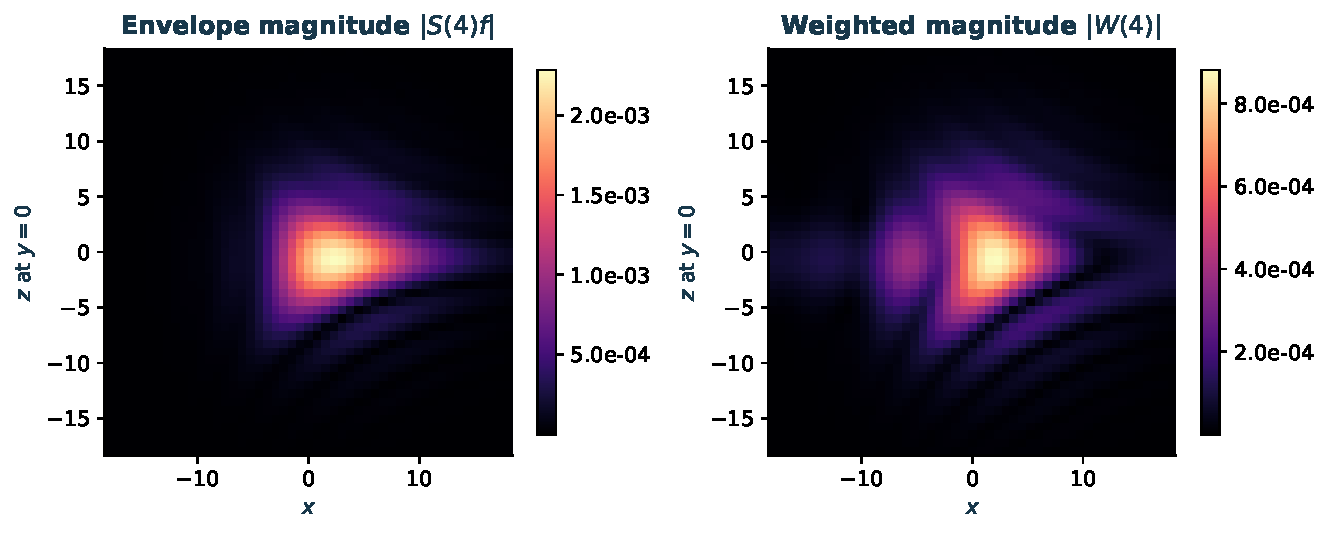
\includegraphics[width=1\linewidth]{visuals/weighted_comparison.pdf}
\caption{Unweighted envelope magnitude and fractionally weighted magnitude for seed 33 at $t=4$.}\label{fig:weight}
\end{figure}

\textbf{Same input, different quantity.} Seed 33 at $t=4$, on the $y=0$ plane.
Each panel has its own amplitude scale. The right panel is the field used in the
inequality; it is not surface elevation or velocity.
\begin{equation}\boxed{R(t;f)=\frac{t^{7/6}\|W(t)\|_\infty}{\|f\|_1}\leq C}\end{equation}
For $\alpha=1/2$, the predicted comparison rate is $t^{-7/6}$. The constant must
be independent of input and time at fixed equation parameters.
\begin{center}\begin{tabular}{ll}\toprule
If the ratio $R(t)$ is\ldots & The weighted peak behaves\ldots\\\midrule
Flat & Like $t^{-7/6}$ over that interval.\\
Falling & Faster than $t^{-7/6}$ over that interval.\\
Rising & Slower than $t^{-7/6}$ over that interval.\\\bottomrule
\end{tabular}\end{center}
\takeaway{The claim is boundedness, not monotonicity. A rising finite curve can
still approach a finite constant. Many inputs make the experiment more searching;
they do not by themselves turn it into a uniform theorem.}


\begin{definition}[Compensated weighted peak]
For nonzero initial data $f\in L^1(\mathbb R^3)$ for which the weighted solution
is bounded, define
\begin{equation}\label{eq:diagnostic}
\mathcal R_{s,\beta}(t;f)
=\frac{t^{7/6}\|\,|D_x+\beta|^{1/2}S_{s,\beta}(t)f\|_{L^\infty(\mathbb R^3)}}
{\|f\|_{L^1(\mathbb R^3)}},\qquad t>0.
\end{equation}
\end{definition}
The notation $R(t;f)$ used below denotes this quantity with the regime understood.
The proposed estimate asserts a constant independent of $t$ and $f$; it does not
assert monotonicity in $t$. Numerical maxima approximate the continuum norm in
\eqref{eq:diagnostic} only to the extent supported by the stated checks.
The primary manuscript is cited as~\cite{MPSdraft}.

\section{Interpretation of the computed fields}

\subsection{Envelope, carrier and intensity}\label{envelope}
The complex envelope carries amplitude and phase. Its magnitude tells us how
large the local oscillations can be; it is not velocity. A carrier supplies the
rapid crests and troughs inside that slowly varying outline.

\begin{figure}[!htbp]\centering
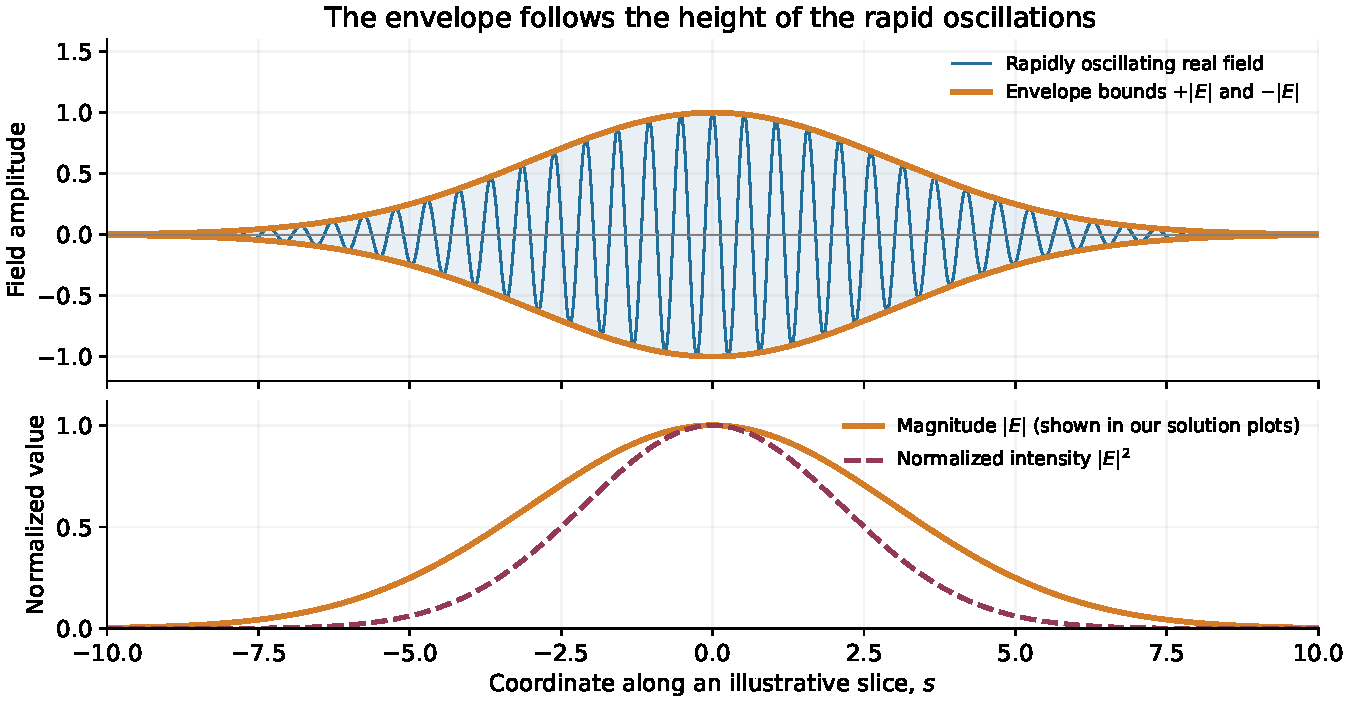
\includegraphics[width=1\linewidth]{figures/envelope_explanation.pdf}
\caption{Envelope magnitude, carrier oscillations and normalized intensity.}\label{fig:envelope}
\end{figure}

\takeaway{The oscillating curve is the wave. The upper and lower outlines are
$+|E|$ and $-|E|$. A magnitude plot shows that outline, without drawing each crest.}
The schematic reconstruction is
\begin{equation}u_{\rm carrier}=\operatorname{Re}\{E\,e^{i\phi_{\rm carrier}}\}.\end{equation}
Phase matters: two envelopes with the same magnitude can produce different crest
positions and different interference. The figures on page \pageref{randomslice} retain the simulated
complex phase and add a visible carrier for illustration.

Optical intensity is proportional to $|E|^2$. A peak magnitude of $0.47$ corresponds
to about $0.22$ of the initial peak intensity when the initial amplitude is one.
Spreading can lower this peak while preserving the integral of $|E|^2$.

\textbf{Units and normalization.} Computations are dimensionless. The early optical
Gaussian examples start at peak one. Canonical decay inputs instead have $L^1=1$.
Their small numerical amplitudes reflect this different normalization and should
not be compared directly with the optical peaks.

\subsection{Illustrative fluid interpretation}\label{fluid}
A group contains several crests: they grow toward its center and fade near its
edges. The envelope is an outline of their amplitude, not another material surface.

\begin{figure}[!htbp]\centering
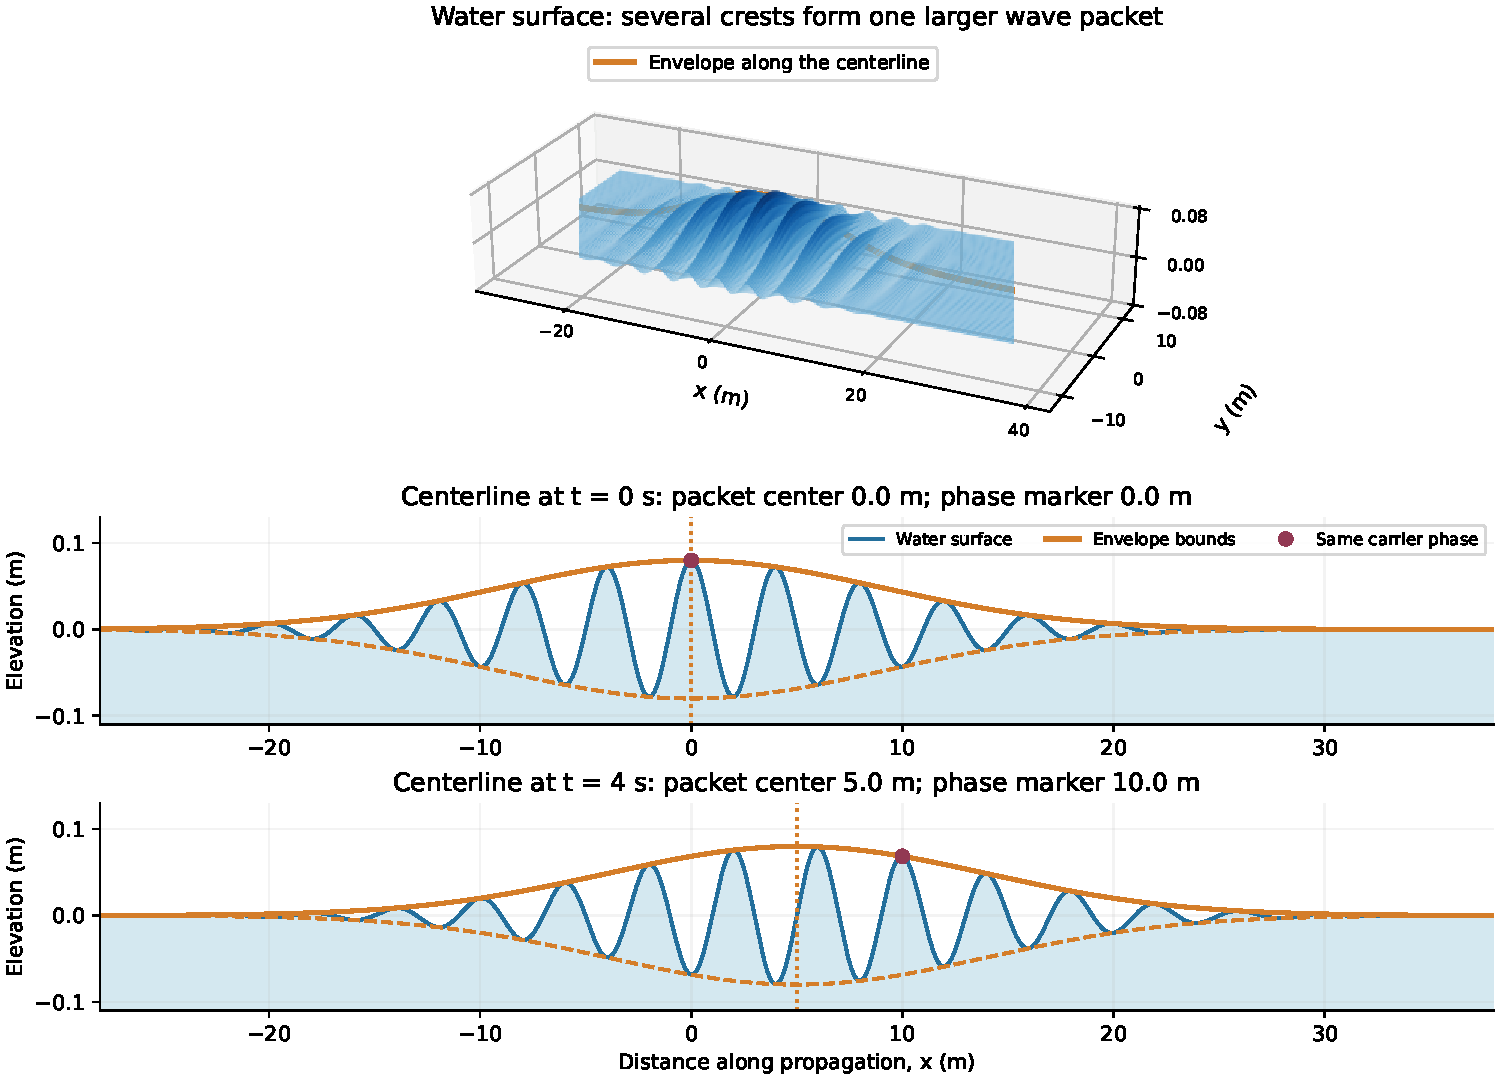
\includegraphics[width=.94\linewidth]{figures/water_packet.pdf}
\caption{Illustrative water-wave packet and the distinction between group and phase motion.}\label{fig:water}
\end{figure}

For small-amplitude deep-water gravity waves, $c_g=c_p/2$: individual crests
move through the group. The dots in the lower panels track phase and group position,
not water parcels. This illustration uses wavelength 4 m and amplitude 0.08 m,
with vertical exaggeration. It omits spreading, nonlinear corrections and breaking.
\takeaway{A surface plot has two horizontal coordinates and elevation. Our 3D
field has three independent coordinates: its amplitude must be shown by color,
slices, or level surfaces, as on the next page.}
{Fluid interpretation: R. Salmon, \href{https://www-pord.ucsd.edu/rsalmon/111.textbook.pdf}{\emph{Introduction to Ocean Waves}}, Chapter 2, pp. 25--26. This is an explanatory analogy, not output from a fluid solver.}

\section{Selected three-dimensional solutions}

\subsection{Random packet: magnitude level surfaces}\label{randomvolume}

\begin{figure}[!htbp]\centering
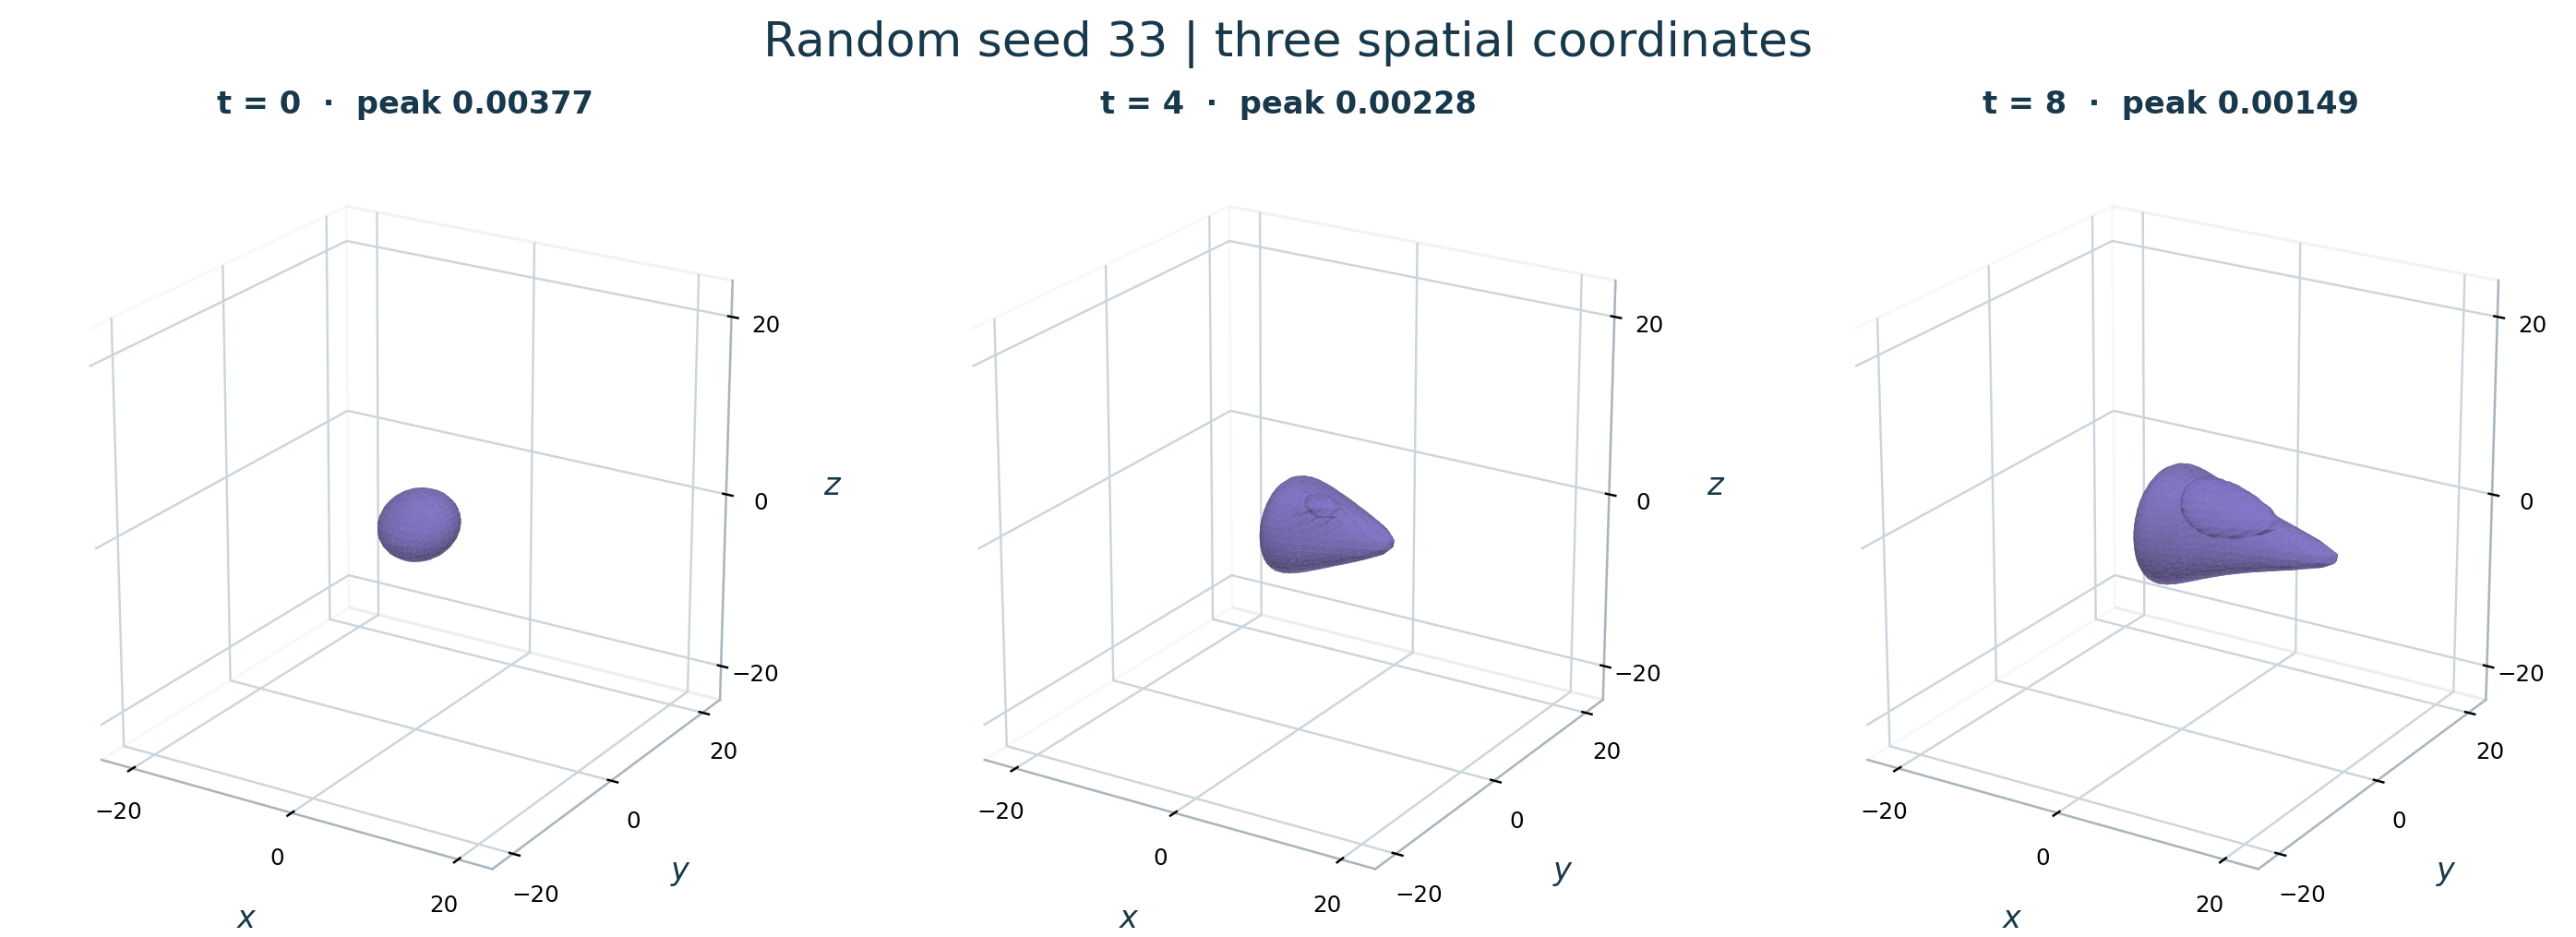
\includegraphics[width=1\linewidth]{../output/figure_review/05_random_seed_33_volumes.png}
\caption{Seed 33: three-dimensional magnitude level surfaces at $t=0,4,8$ (review-collection figure 5).}\label{fig:randomvolume}
\end{figure}

These are surfaces
of $|u|=0.3\max|u|$, using the full sampled maximum separately at each time.
All axes are spatial coordinates, and every panel uses the same $[-24,24]^3$
viewing cube. The magnitude is represented by the surface threshold, not by a
vertical elevation axis. The numerical maxima appear above the panels.

The initially compact central region becomes elongated and asymmetric. The
geometry changes while the sampled maximum drops from approximately $0.00377$
to $0.00149$. Because the threshold also falls, the growing visible region cannot
be interpreted as an increase of amplitude or as a quantitative measure of volume.
\callout{\textbf{Main observation.} The two selected fields illustrate different
routes to a lower peak: deformation of a random envelope and overlap of two
phase-offset packets. Their figures describe shape; the diagnostic comparison
on page \pageref{selecteddiag} measures amplitude and its relation to the decay question.}

\subsection{Random packet: slices and carrier reconstruction}\label{randomslice}
The first input combines twelve complex plane waves under a Gaussian window:
\begin{equation}
 f_{33}(X)=\frac{e^{-|X|^2/18}}{Z_{33}\sqrt{12}}
 \sum_{j=1}^{12}e^{i(q_j\cdot X+\phi_j)},\qquad X=(x,y,z).
\end{equation}
The wavevectors are sampled from independent centered normal components with
standard deviation $0.25$; phases are uniform on $[0,2\pi)$. NumPy seed 33 fixes
the realization. The positive constant $Z_{33}$ normalizes the sampled $L^1$ norm
to one. This is one reproducible realization, not a statistical ensemble average.

\begin{figure}[!htbp]\centering
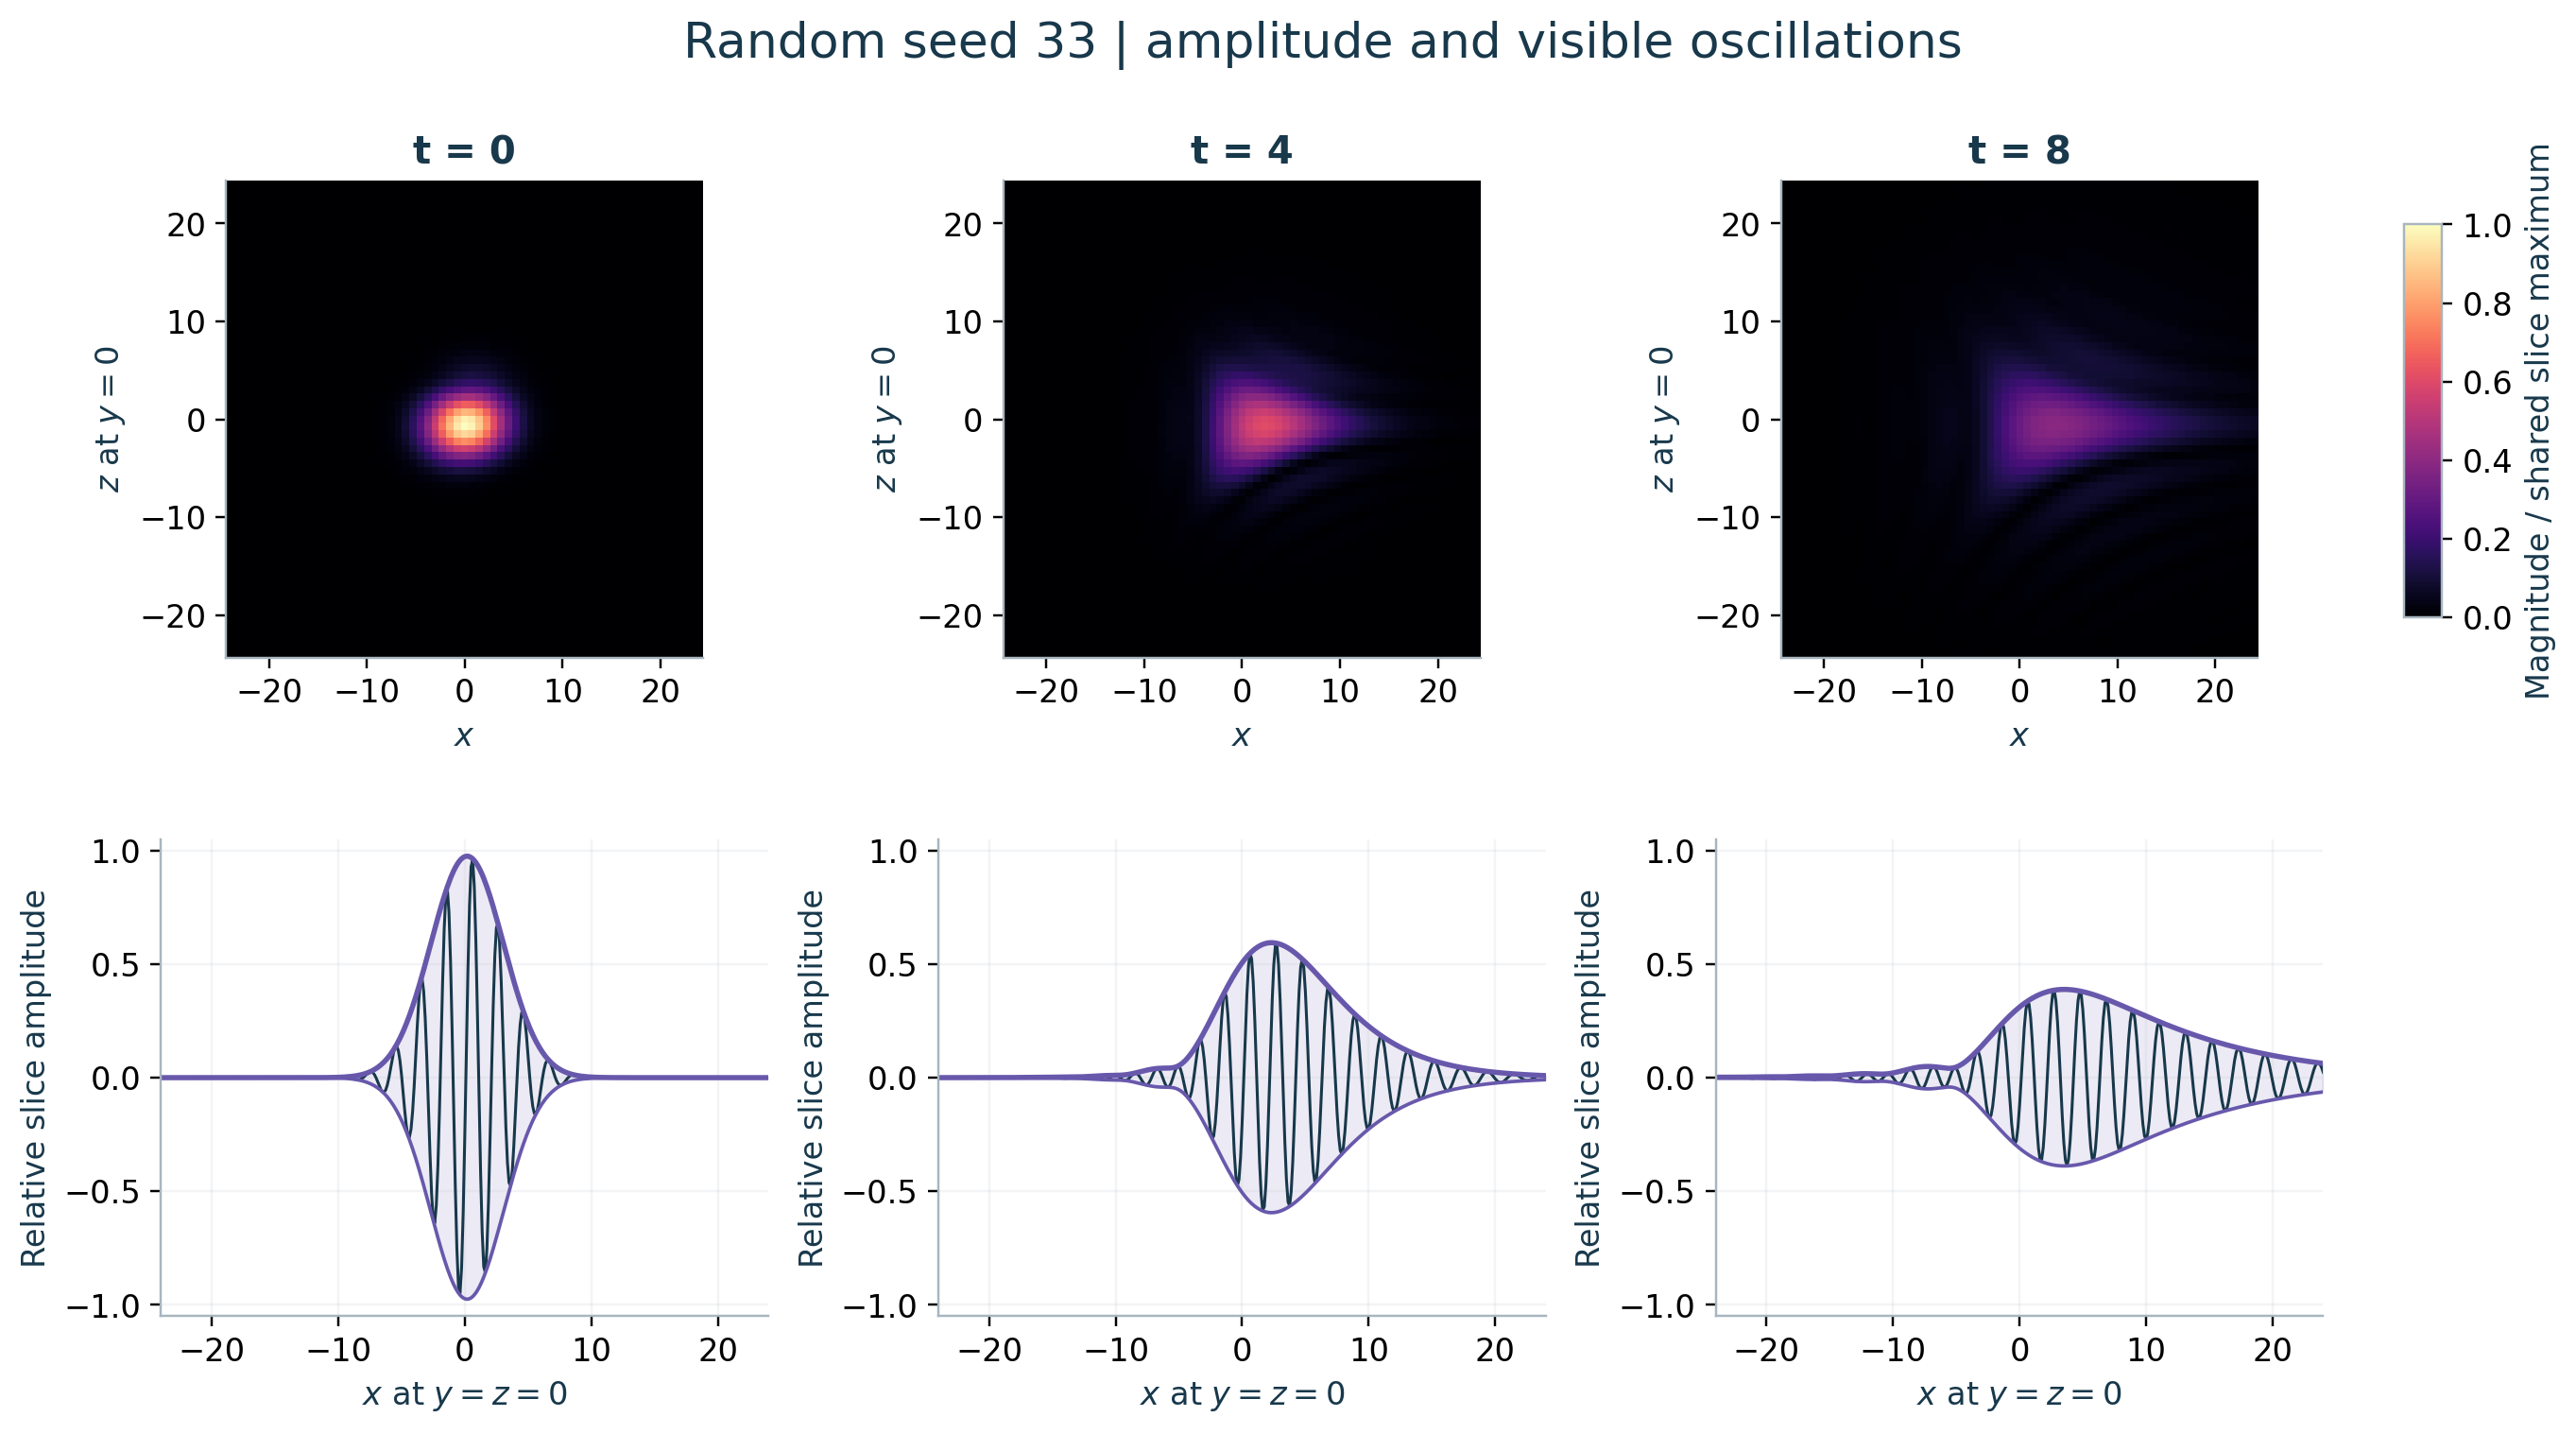
\includegraphics[width=1\linewidth]{../output/figure_review/06_random_seed_33_slices_and_waves.png}
\caption{Seed 33: planar magnitude slices and illustrative carrier traces (review-collection figure 6).}\label{fig:randomslice}
\end{figure}

Top panels show
$|u(x,0,z,t)|$. Their shared color scale divides by the largest displayed slice
magnitude across the three times. Bottom panels show the centerline envelope
$\pm|u(x,0,0,t)|$ and the illustrative carrier reconstruction
$\operatorname{Re}\{u(x,0,0,t)e^{3ix}\}$, divided by the same constant.

The fixed color scale makes the reduction of the bright central region visible.
The later slices also reveal weaker oscillatory structure away from the center.
Those lower-amplitude features are largely absent from the 30\% level surfaces
in Figure~\ref{fig:randomvolume}: a slice and a level surface answer different questions.

The dark oscillations remain inside the positive and negative envelope. Their
locations depend on the phase of the complex solution as well as on the added
carrier. The complex centerline is Fourier-interpolated from spacing $0.75$ to
$0.125$ for drawing; this makes the reconstruction smooth without adding simulated
Fourier modes. The carrier wavenumber 3 is an illustrative choice.
\callout{\textbf{Reading the magnitude.} It is dimensionless envelope amplitude,
not velocity. Neither these oscillations nor the 3D level surfaces represent a
calibrated water elevation. A physical surface reconstruction would require a
specified water-wave model and physical scales.}

\subsection{Two phase-offset packets: linear interference}\label{pairvolume}
The second input is deliberately simpler than the random realization:
\begin{equation}
 f_{\rm pair}(X)=\frac{1}{Z_{\rm pair}}
 \left[e^{-((x+5)^2+y^2+z^2)/18}
       +0.7i\,e^{-((x-5)^2+y^2+z^2)/18}\right].
\end{equation}
The packet centers begin at $x=-5$ and $x=5$. Each has width 3; the second has
relative amplitude $0.7$ and a phase offset of $\pi/2$. As before, $Z_{\rm pair}$
is chosen using the grid quadrature so that the initial $L^1$ norm is one.

\begin{figure}[!htbp]\centering
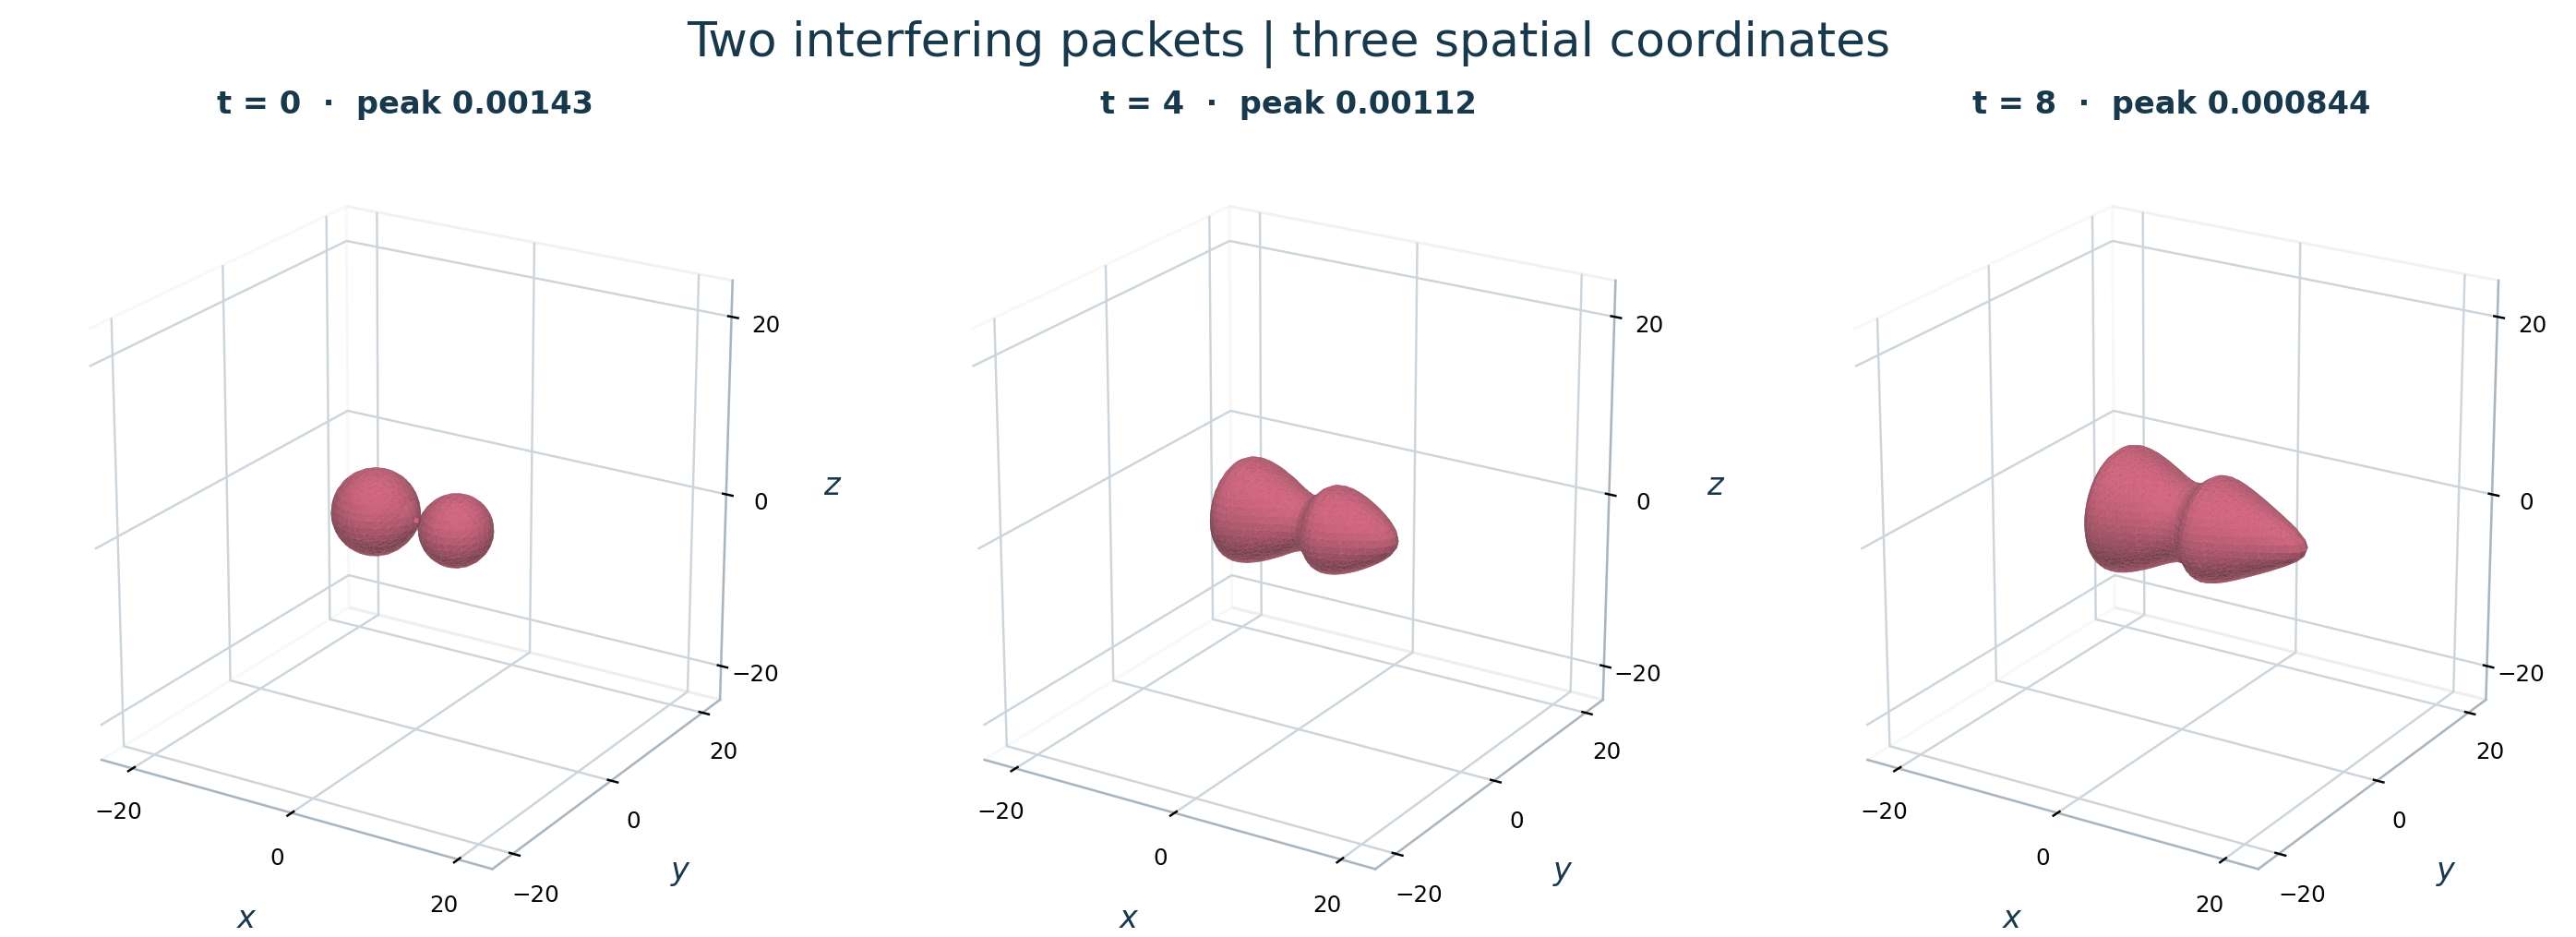
\includegraphics[width=1\linewidth]{../output/figure_review/07_two_interfering_packets_volumes.png}
\caption{Two phase-offset packets: magnitude level surfaces at $t=0,4,8$ (review-collection figure 7).}\label{fig:pairvolume}
\end{figure}

The same 30\%-of-current-peak
rule and spatial viewing cube are used as in Figure~\ref{fig:randomvolume}. The separated initial
regions develop an overlapping, asymmetric shape. The plots show thresholded
magnitude geometry; they do not track individual fluid parcels.

The sampled peak decreases from $0.00143$ to $0.000844$, a smaller relative drop
than for the random packet over the same interval. Both inputs have $L^1=1$, but
they have different initial peaks, $L^2$ norms, and spectra. Equal $L^1$ normalization
therefore does not make their initial pointwise amplitudes equal.

\textbf{Why phase matters even in a linear model.} Let $u_1$ and $u_2$ denote the
evolved, normalized components, including the factor $0.7i$ in $u_2$. Linearity gives
\begin{equation}
 u=u_1+u_2,\qquad
 |u|^2=|u_1|^2+|u_2|^2+2\operatorname{Re}(u_1\overline{u_2}).
\end{equation}
The last term is interference. Initially the Gaussian components have a quadrature
phase offset, so that term vanishes. Their subsequent complex evolution can make
it nonzero. The overlapping magnitude thus need not be the sum of the two separate
magnitudes.
\callout{\textbf{Interpretation.} This is linear superposition with interference.
The apparent joining of level surfaces is not evidence of nonlinear attraction,
soliton interaction, or irreversible merger.}

\subsection{Two-packet slices and carrier reconstruction}\label{pairslice}
The planar and centerline views show the same two-packet computation from a more
familiar perspective. The two initial amplitude peaks become less distinct as
their evolved fields overlap, while the carrier oscillations remain visible.

\begin{figure}[!htbp]\centering
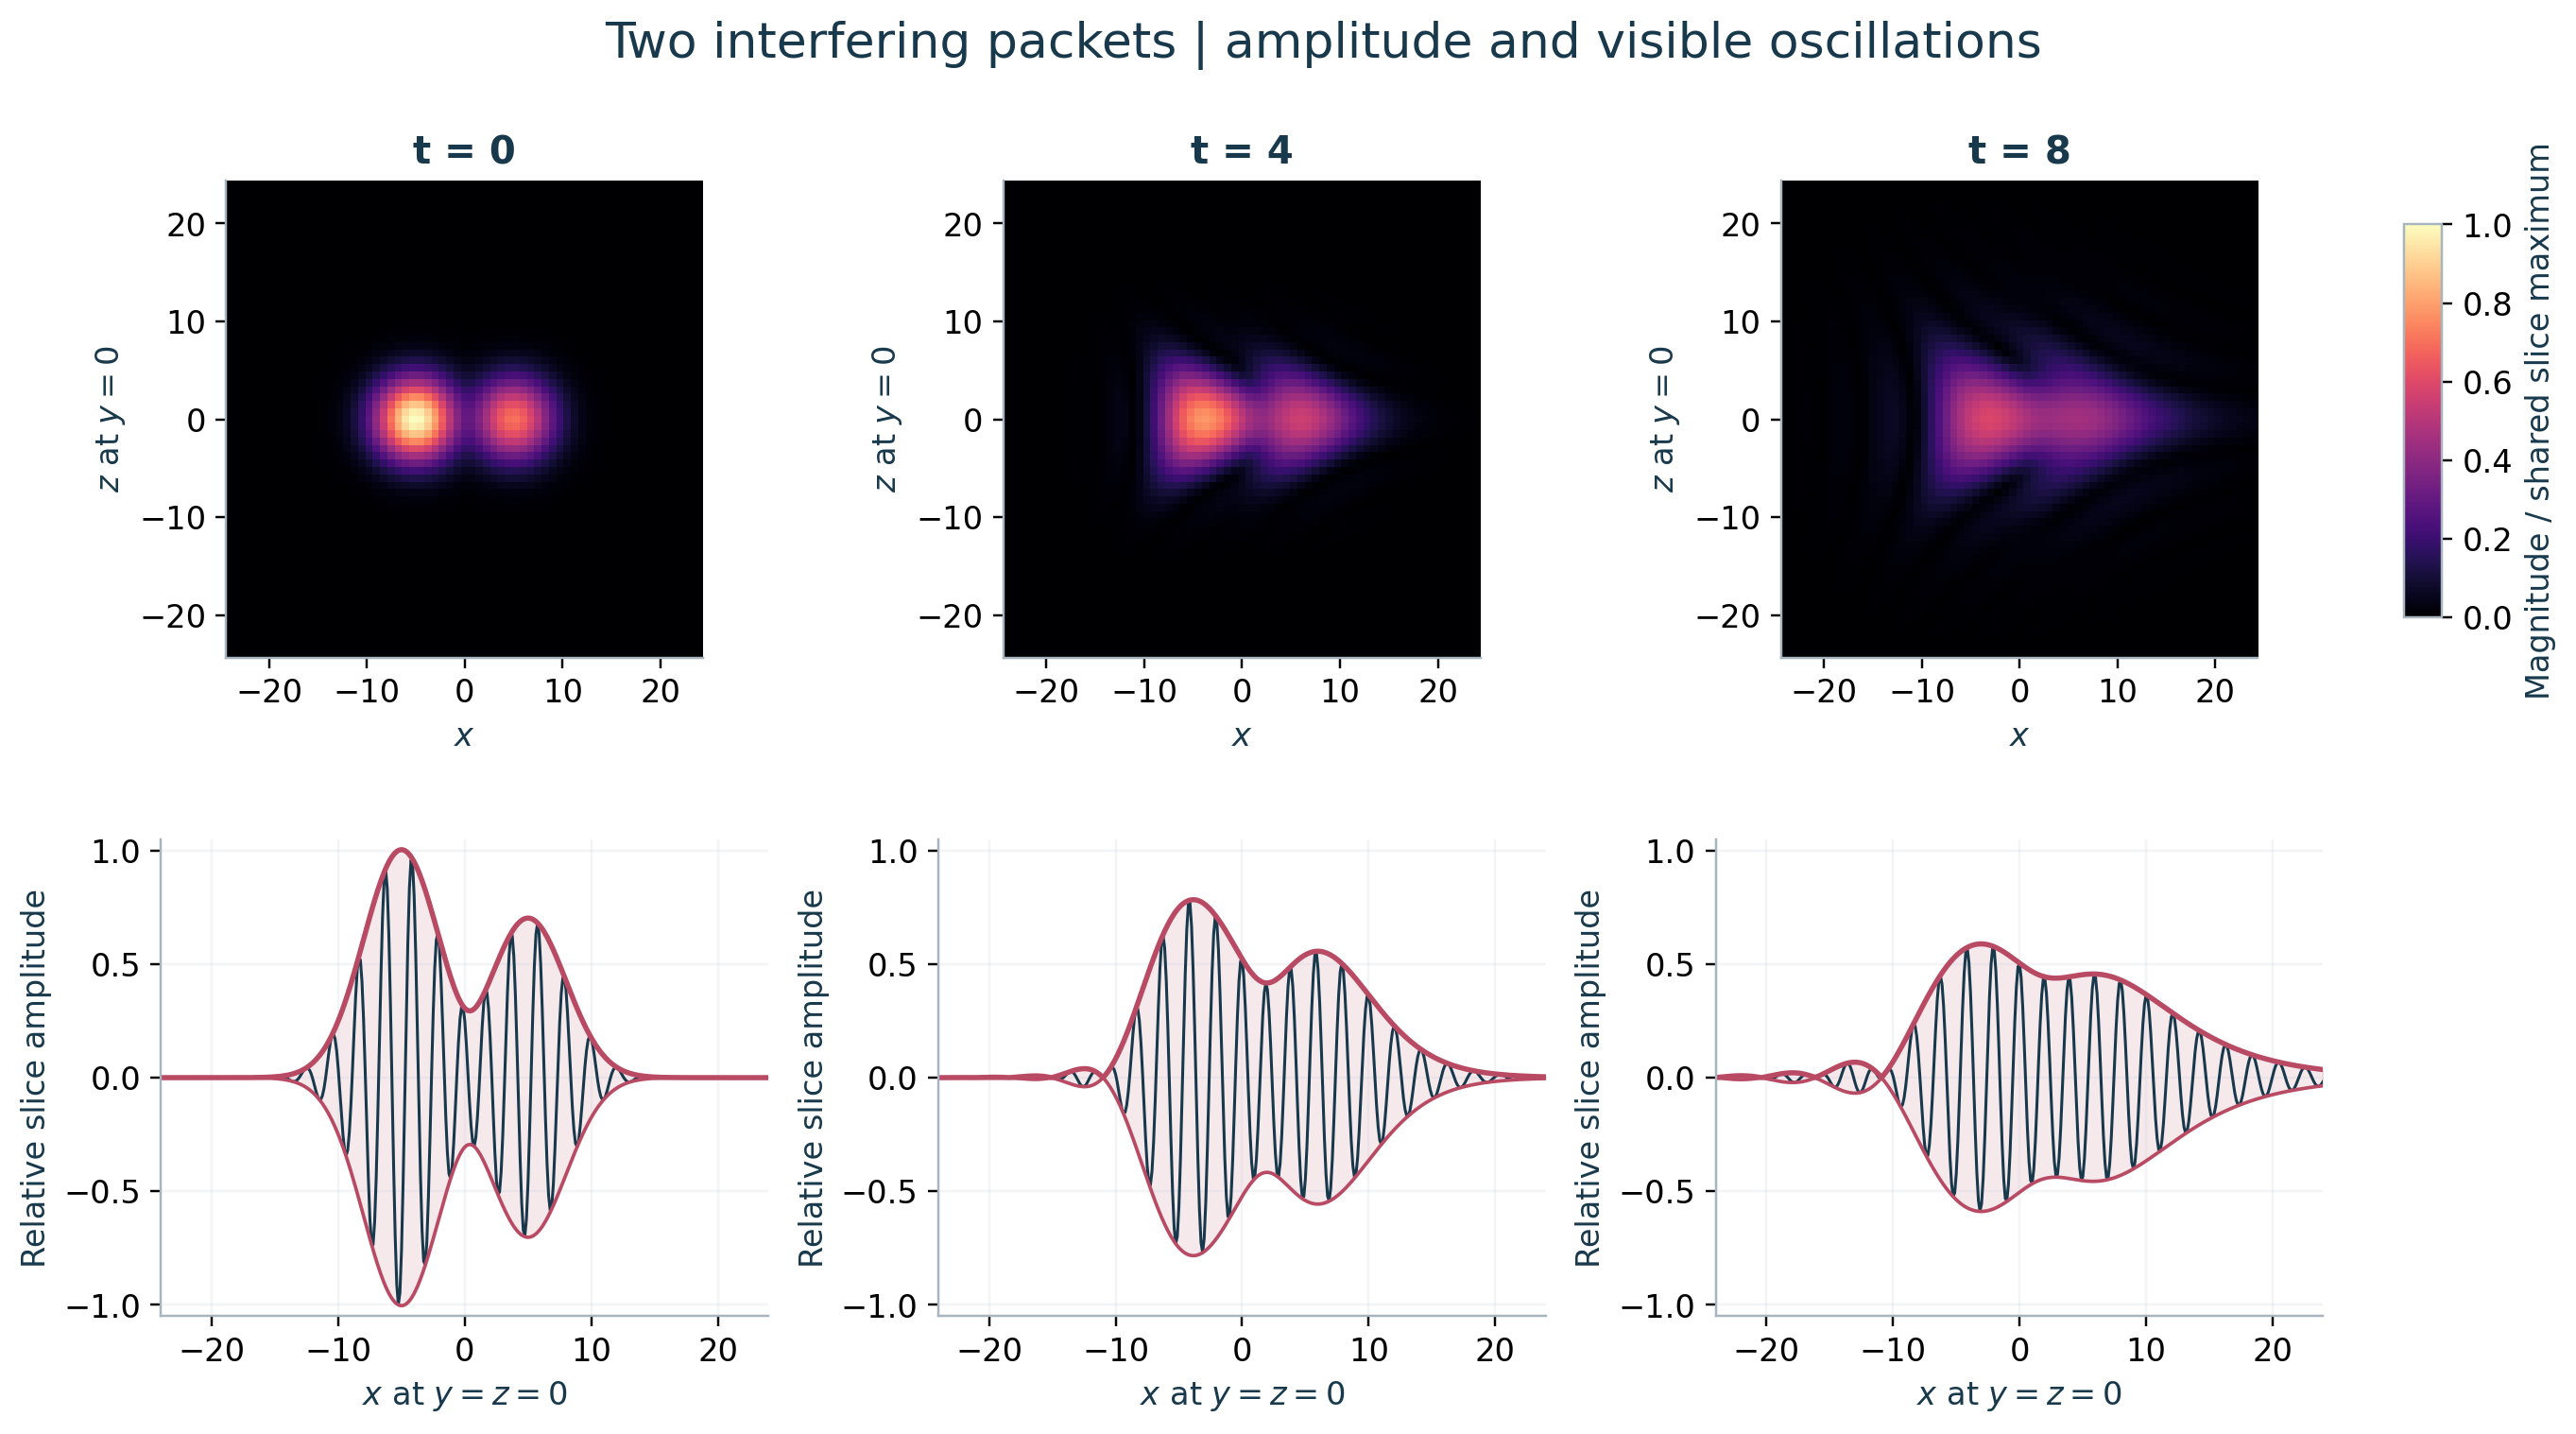
\includegraphics[width=1\linewidth]{../output/figure_review/08_two_interfering_packets_slices_and_waves.png}
\caption{Two phase-offset packets: planar slices and carrier traces (review-collection figure 8).}\label{fig:pairslice}
\end{figure}

The conventions are identical to Figure~\ref{fig:randomslice}, but the normalization divisor is
computed separately for this case. Colors can be compared across times within
this figure; they cannot be used for an absolute amplitude comparison with
Figure~\ref{fig:randomslice}. The printed full-volume peaks and the table on page \pageref{selecteddiag} provide that comparison.

The upper panels retain the weaker structures below the threshold used in Figure~\ref{fig:pairvolume}.
The bottom row displays $\pm|u|$ as an outline rather than as an additional physical
wave. The dark curve combines the simulated phase with the illustrative carrier;
its crests are not numerical grid markers or tracked particles.

\textbf{What the comparison reveals.} The random realization begins with a more
concentrated peak and loses a larger fraction of that peak. The two-packet profile
spreads and overlaps while retaining a broader region of visible amplitude.
These differences persist despite identical evolution rules and initial $L^1$
normalization. Initial phase and spectral content are therefore essential parts
of the experiment definition.

\textbf{What the comparison cannot decide.} The figures do not determine a
universal decay constant, establish monotonicity for arbitrary data, or predict
which profile will have the larger compensated ratio at much later times. A
centerline may also miss an off-axis maximum. The following diagnostics therefore
search the entire simulated volume rather than one selected slice.
\callout{\textbf{Why these figures are paired.} Figures~\ref{fig:randomvolume} and~\ref{fig:pairvolume} establish
the three-dimensional geometry. Figures~\ref{fig:randomslice} and~\ref{fig:pairslice} explain the amplitude and phase
behind that geometry. Keeping each volume next to its companion slice avoids
asking one visualization to communicate both shape and decay.}

\subsection{Amplitude and weighted diagnostics}\label{selecteddiag}
For the same two inputs and the same grid, we evaluate 17 times from 0 to 8.
The weighted field and compensated ratio are
\begin{equation}
 W(t)=|D_x|^{1/2}S(t)f,\qquad
 R(t;f)=\frac{t^{7/6}\|W(t)\|_\infty}{\|f\|_1}.
\end{equation}
These are different from the unweighted envelope magnitudes shown in Figures~\ref{fig:randomvolume}--\ref{fig:pairslice}.
The ratio is displayed only for $t>0$.

\begin{figure}[!htbp]\centering
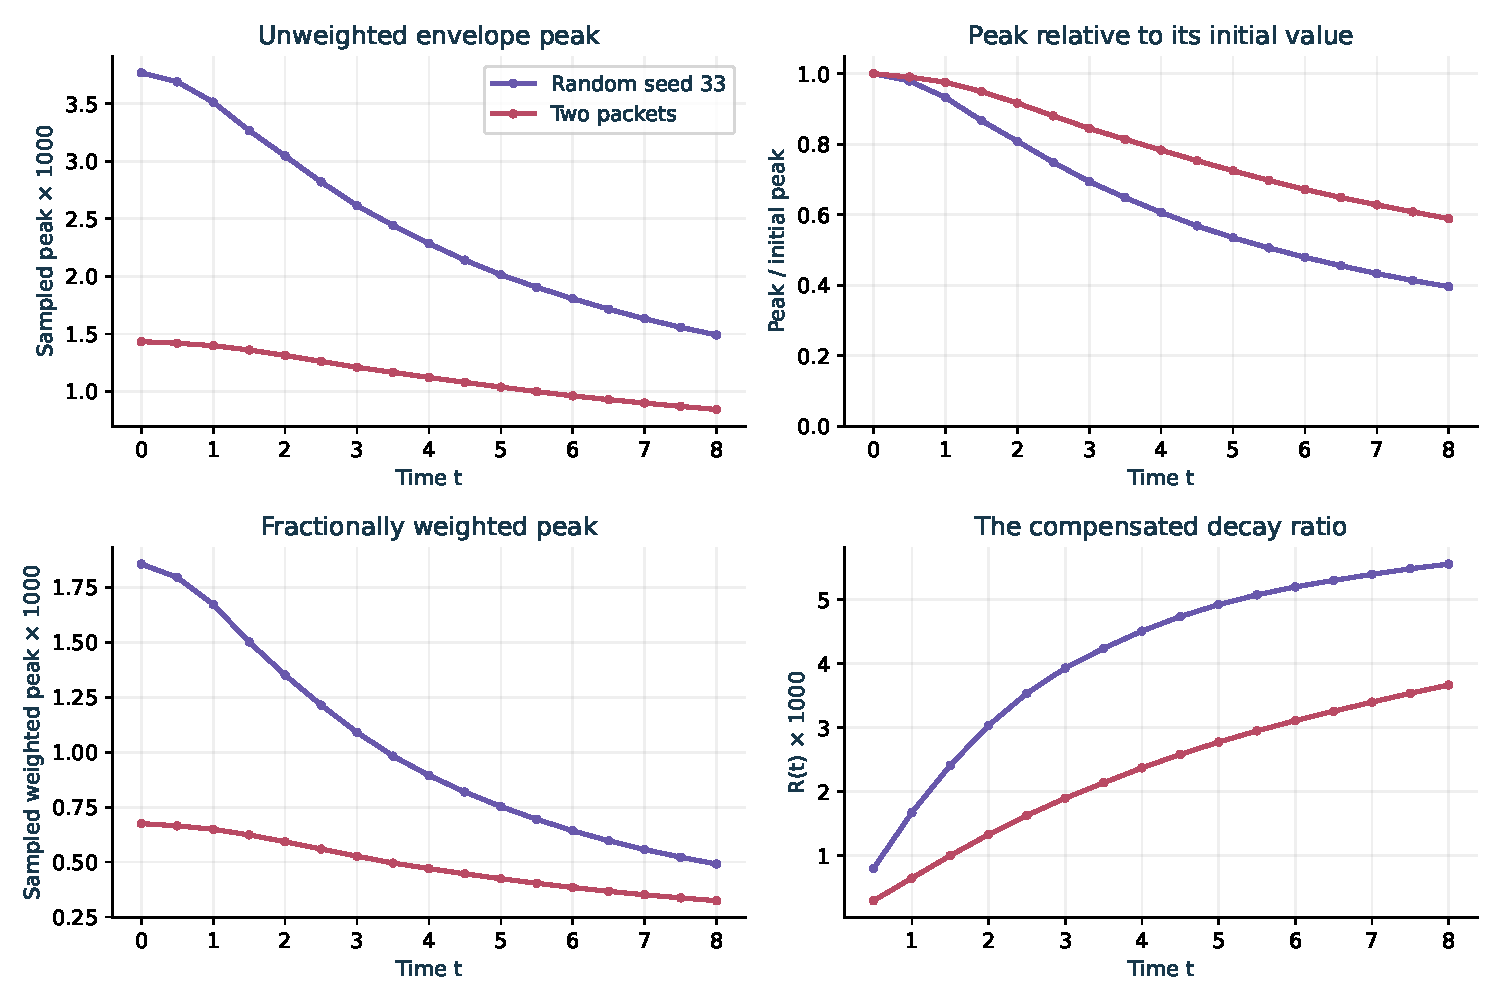
\includegraphics[width=1\linewidth]{../results/selected_packets/comparison.pdf}
\caption{Unweighted and weighted diagnostics for the two selected inputs.}\label{fig:diagnostics}
\end{figure}

Maxima are
sampled over the full periodic volume. The upper right panel removes the difference
in initial peak height. The lower right panel measures the quantity associated
with the manuscript's $\alpha=1/2$, $p=\infty$ bound.
\begin{center}\small\begin{tabular}{lrrrr}\toprule
Input & Peak at 0 & Peak at 8 & Peak reduction & $R(8)$\\\midrule
\SelectedRows\bottomrule\end{tabular}\end{center}
\callout{\textbf{The relevant distinction.} A decreasing unweighted peak can
coexist with an increasing compensated ratio. The proposed inequality asks
whether $R(t;f)$ stays below an input-independent constant, not whether every
finite curve decreases.}
All curves in this experiment are measurements on one finite grid. Their purpose is to
connect the selected visuals to the research question; they are not a new
convergence study or an asymptotic fit.

\section{Decay experiments and spatial reliability}

\subsection{Initial survey of eleven input families}\label{survey}

\begin{figure}[!htbp]\centering
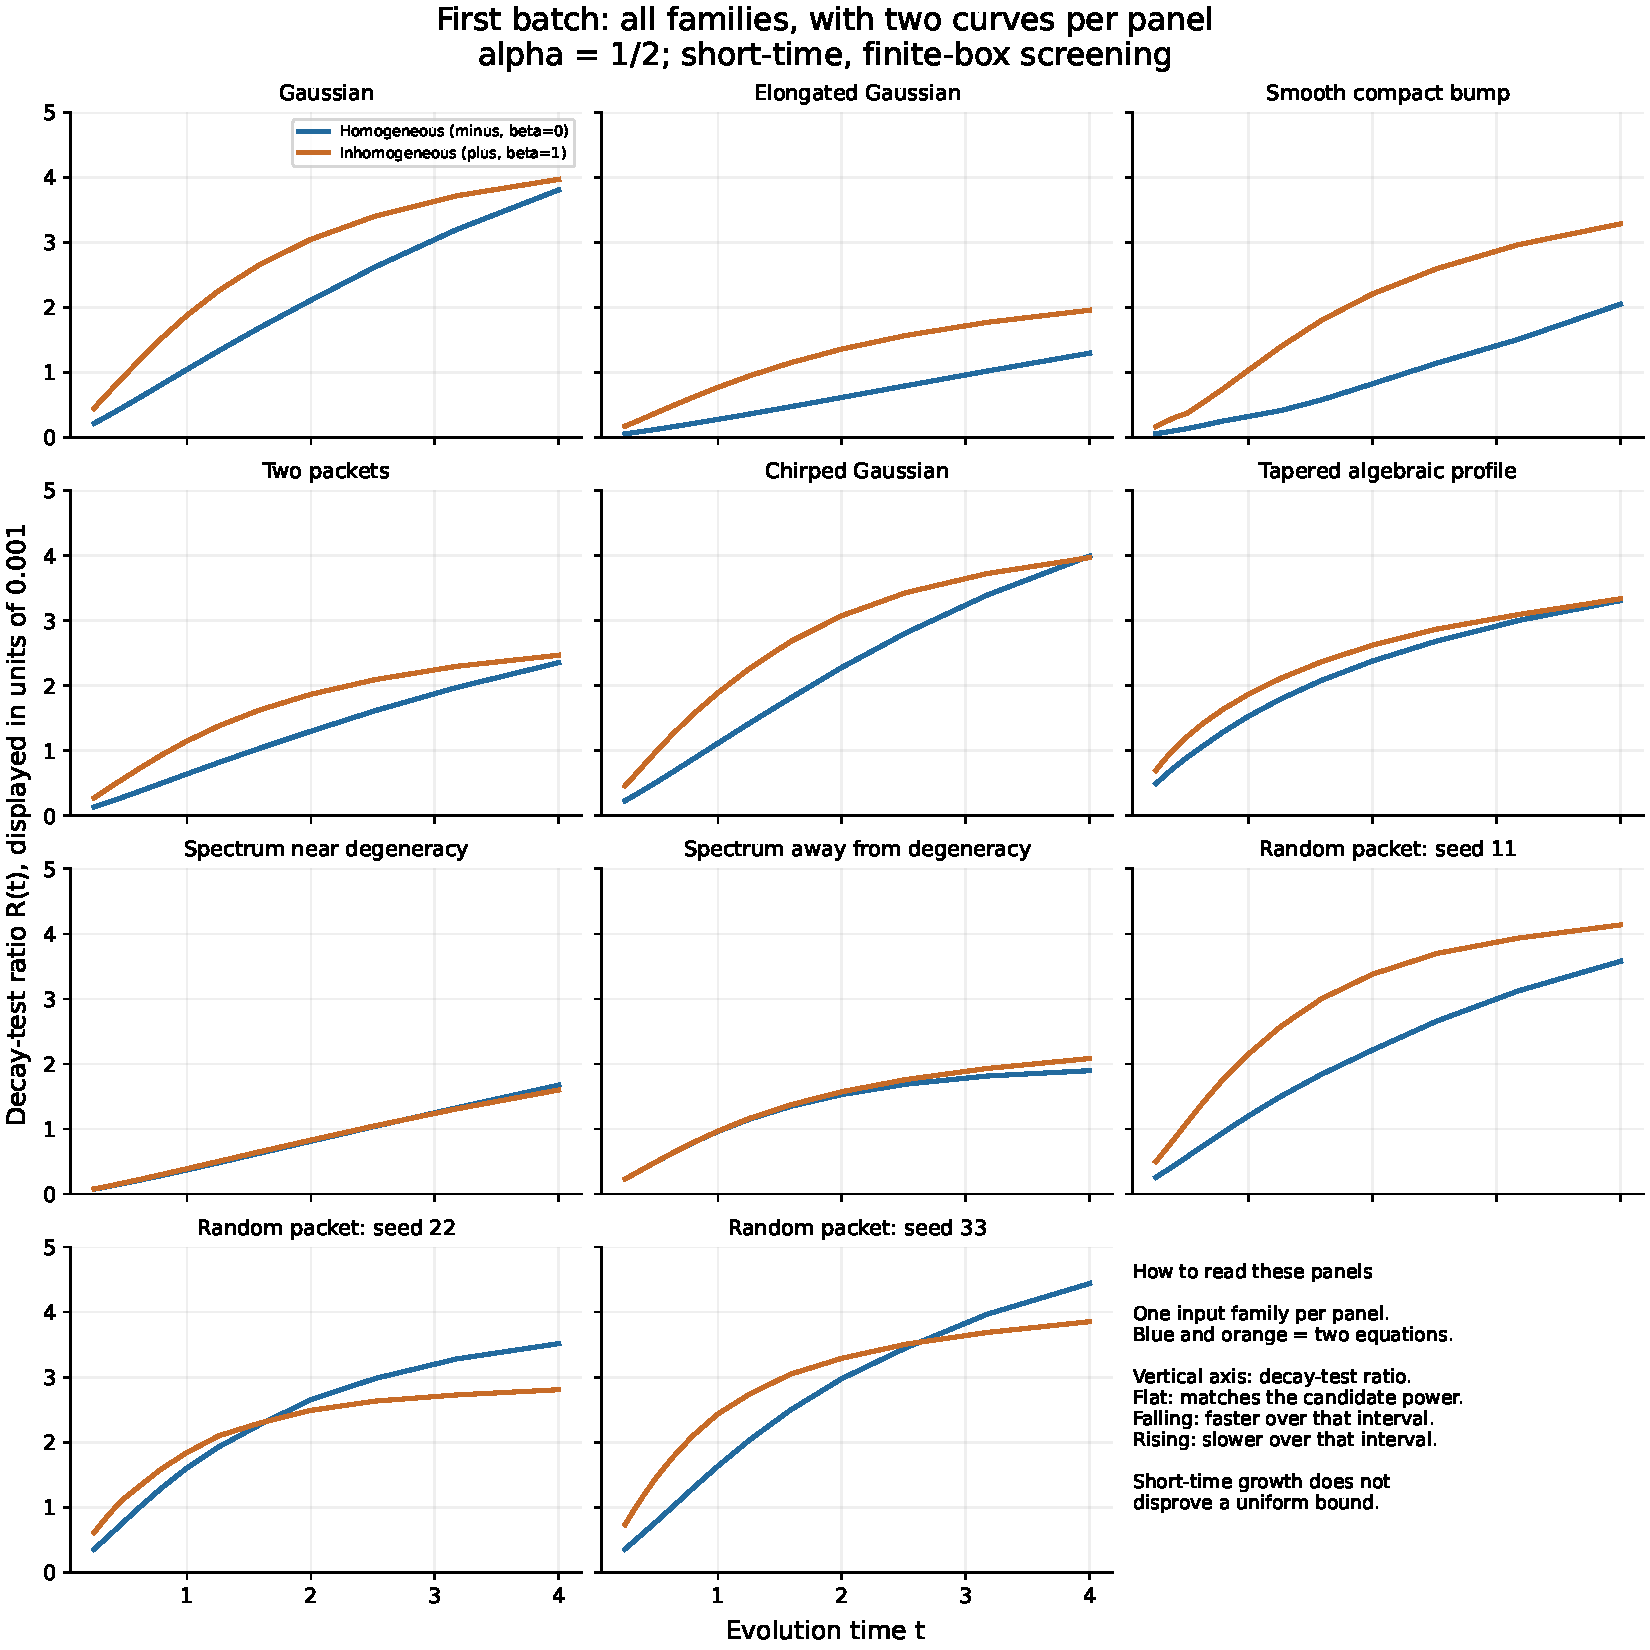
\includegraphics[width=.98\linewidth]{../results/decay_dataset/families_clear.pdf}
\caption{Initial eleven-family weighted-decay survey in two canonical regimes.}\label{fig:survey}
\end{figure}

{\small Original short-time survey: two equation regimes per panel, $\alpha=1/2$,
length-96 box. These curves remain exploratory finite-box measurements. Recipes
include compact, anisotropic, chirped, tapered algebraic and random inputs.
The three random seeds shown earlier belong to this collection. No measured
fluid dataset has been imported.}

\subsection{Intermediate-time refinement}\label{refined}

\begin{figure}[!htbp]\centering
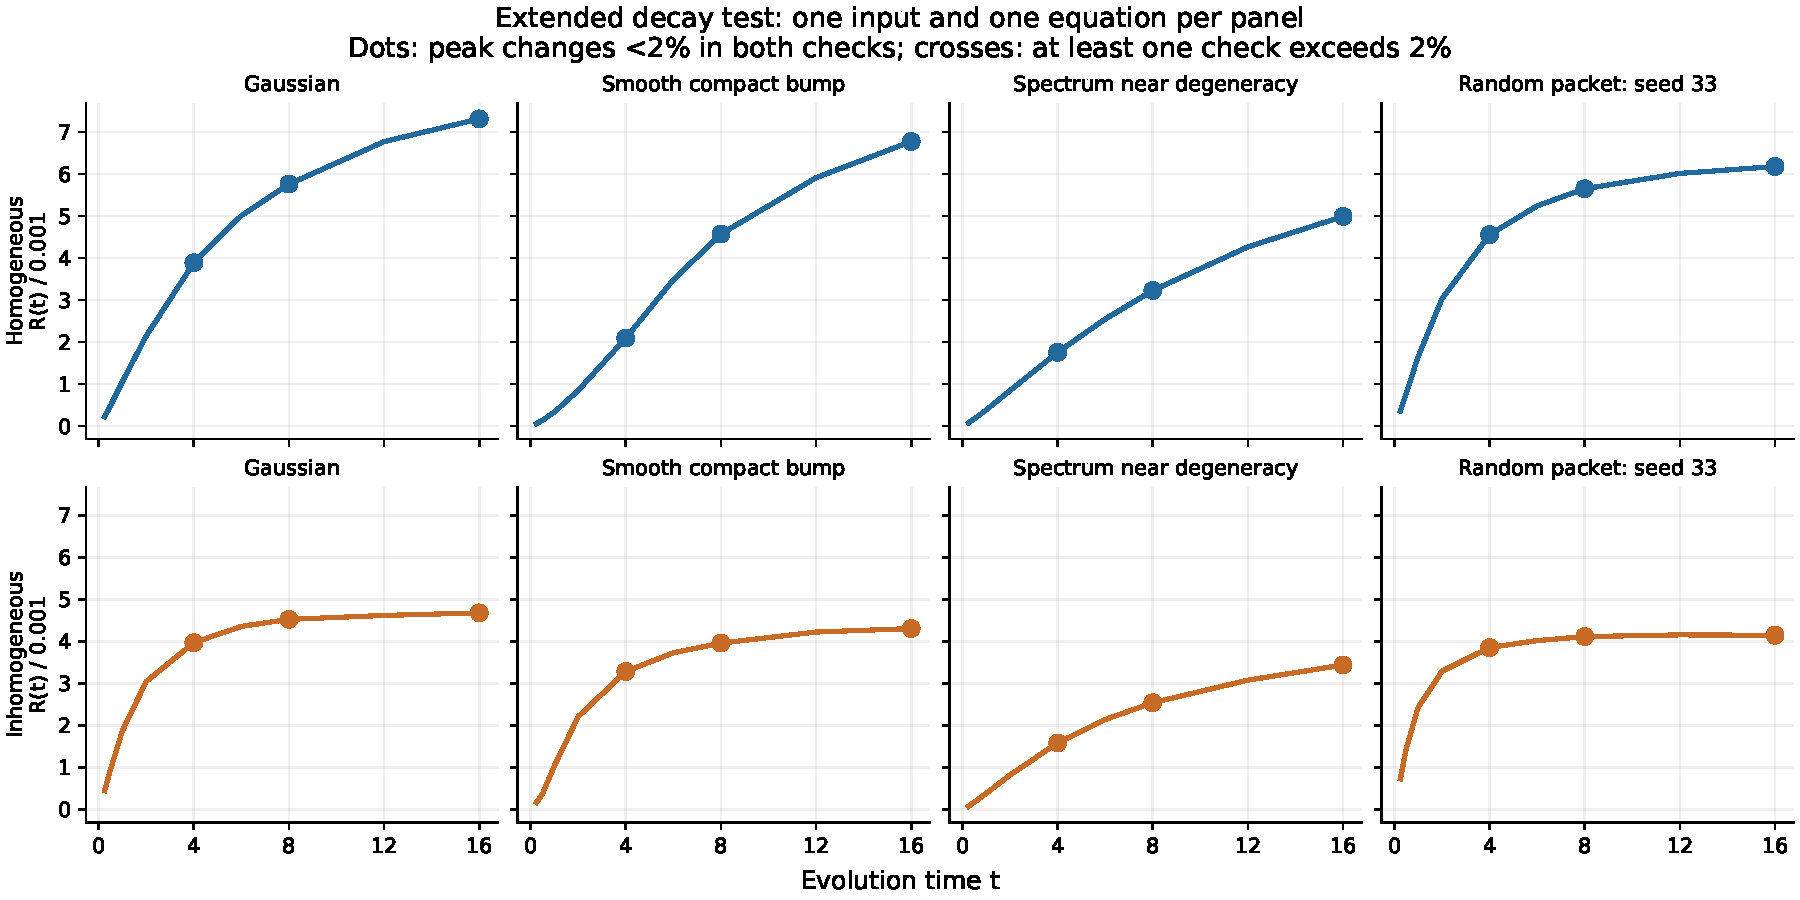
\includegraphics[width=1\linewidth]{../results/decay_dataset/refined_clear.pdf}
\caption{Intermediate-time weighted-decay curves and refinement checks through $t=16$.}\label{fig:refined}
\end{figure}

Curves use a length-288 cube at spacing 1. Dots identify the checked times
$t=4,8,16$ passing the exploratory 2\% peak-change screen in both domain and grid
comparisons; intermediate times were not independently checked.
\takeaway{Across 24 checked case--time combinations, the largest domain peak
change is 1.62\% and the largest grid peak change is 0.94\%. This supports the
intermediate-time comparisons, with weaker tolerances than the four-case endpoint audit.}
\textbf{Next scientific step.} Extend the reliable time window for more recipes,
keeping input normalization fixed and testing spatial stability at each new stage.
A candidate contradiction needs sustained growth that survives those checks;
strengthening a uniform theorem needs an argument covering its full input class.

\subsection{Gaussian-based computations through $t=256$}\label{longresults}

\begin{figure}[!htbp]\centering
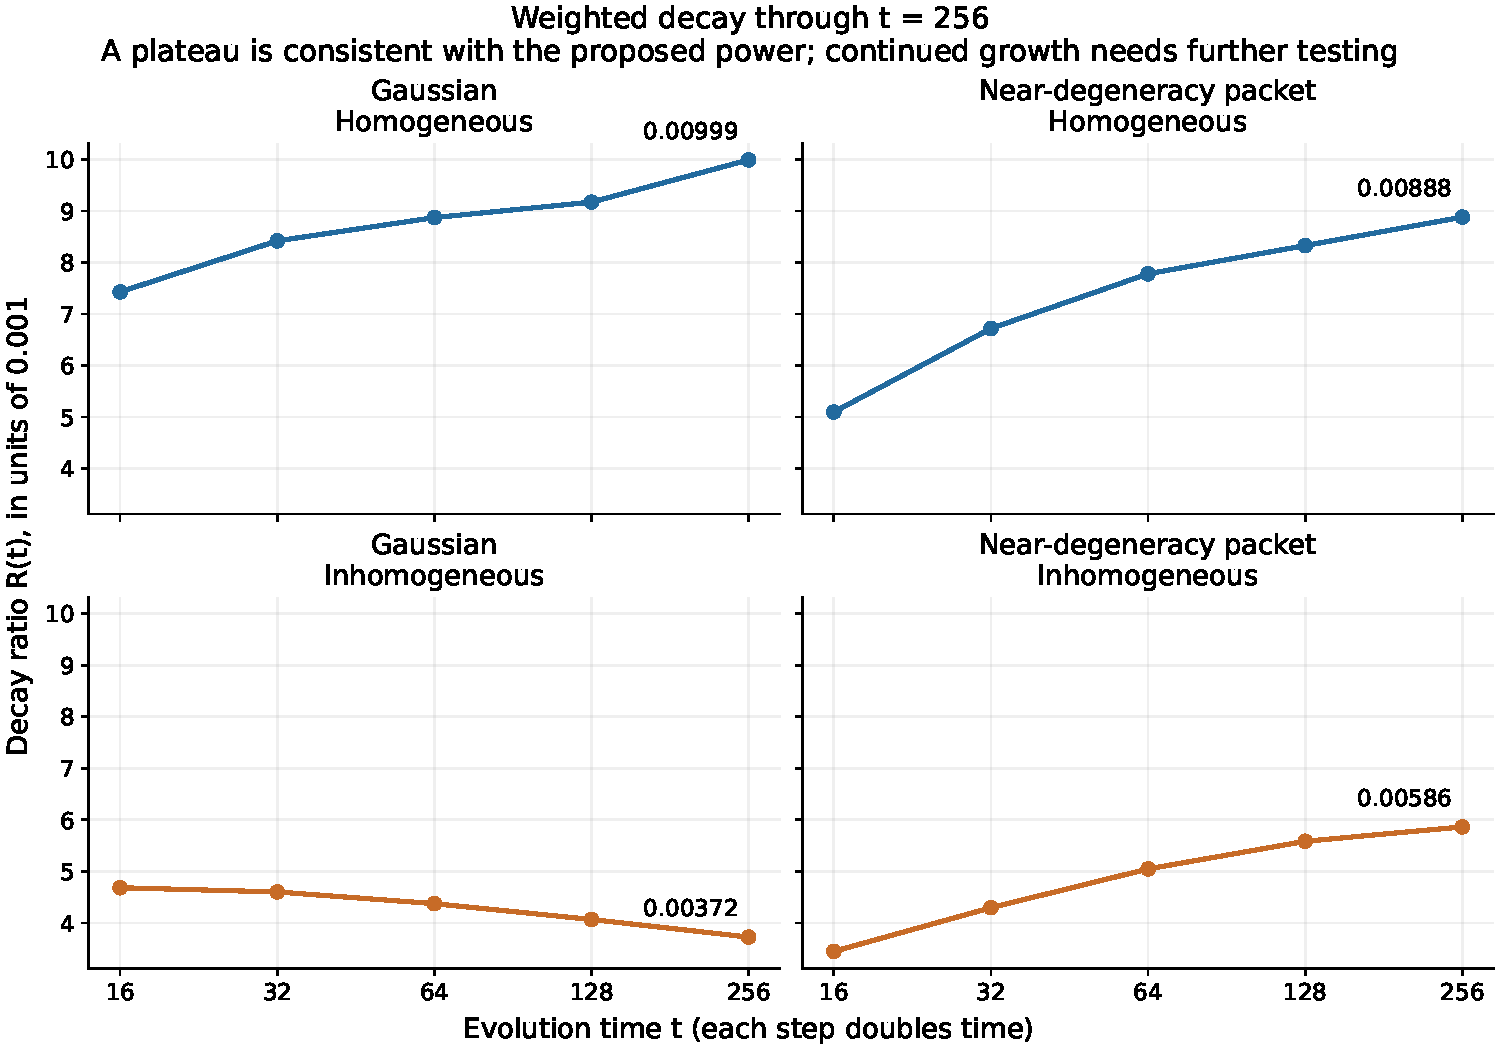
\includegraphics[width=1\linewidth]{../results/long_time/decay_256.pdf}
\caption{Compensated weighted peaks for four Gaussian-based cases through $t=256$.}\label{fig:long}
\end{figure}

The inhomogeneous Gaussian ratio falls at late times; the other three rise over
the last doubling. Those are finite-time trends, not asymptotic conclusions.
\begin{center}\small\begin{tabular}{llrrr}\toprule
Equation & Input & $R(128)$ & $R(256)$ & Local exponent\\\midrule
\LongRows\bottomrule\end{tabular}\end{center}
The exponent is $-\log[M(256)/M(128)]/\log2$, where $M=\|W\|_\infty$.
Compare it with $7/6\simeq1.167$; it describes one time doubling only.
These curves and entries retain the long-time batch values. The subsequent audit refines the four endpoint ratios on page \pageref{spatialaudit}.
\takeaway{We now have a longer observation window. The strongest result is the
improved reliability of its four endpoint peaks, shown next. No counterexample
or stronger uniform exponent has been established.}

\subsection{Spatial stability of candidate maxima}\label{reliability}
At fixed $t=256$, we increased the longitudinal period from 32,768 to 65,536 and
then 131,072. Separately, the radial search grew from 2,048 to 4,096. The broad
search retained $\Delta x=0.25$ and $\Delta r=2$, followed by local peak optimization.

\begin{figure}[!htbp]\centering
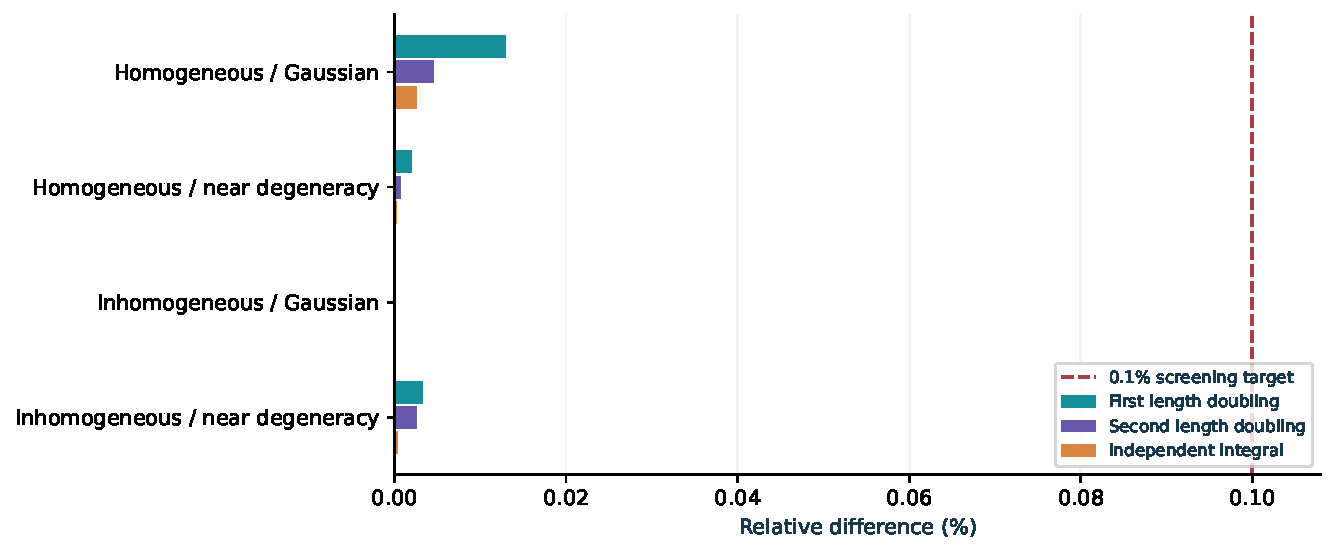
\includegraphics[width=1\linewidth]{visuals/reliability.pdf}
\caption{Relative changes in candidate weighted peaks under the spatial audit at $t=256$.}\label{fig:reliability}
\end{figure}

\takeaway{All four cases pass the 0.1\% numerical screen. The largest final
change in refined peak magnitude is 0.00459\%; the largest location drift is
0.00079 spatial units.}
An independent non-periodic integral agrees within 0.0026\% at the candidate peaks.
Extending the radial search found no larger sampled maximum. These checks support
stability under the tested changes, rather than supplying a rigorous error bound.

\textbf{Why length matters.} The inhomogeneous near-degeneracy peak is near
$x=-841$ at $t=256$. It lies far outside the length-288 box used for the earlier
experiments. A long-time curve on that old box could confuse periodic recirculation
with whole-space behavior.

\textbf{What remains unresolved.} A finite search and local refinement can miss a
narrow or distant maximum. This audit covers four Gaussian-based cases at one time
and one derivative weight. It does not transfer automatically to random inputs.

\section{Experiments motivated by analytical structure}

\subsection{Cubic scaling and its numerical verification}\label{research}
The literature review suggested replacing a purely visual search with experiments
that target the structure of the dispersion. We begin with an exact symmetry of
the homogeneous equation, then vary spectral geometry and cancellation, and test
an independent integral calculation.
\begin{equation}
 f_\lambda(X)=\lambda^3 f(\lambda X),\qquad \|f_\lambda\|_1=\|f\|_1,
 \qquad R(t;f_\lambda)=R(\lambda^3t;f).
\end{equation}
Here $X=(x,y,z)$ and $\beta=0$. At $t=8/\lambda^3$, all three rescaled
inputs should produce the same compensated ratio as the original at $t=8$.

\begin{figure}[!htbp]\centering
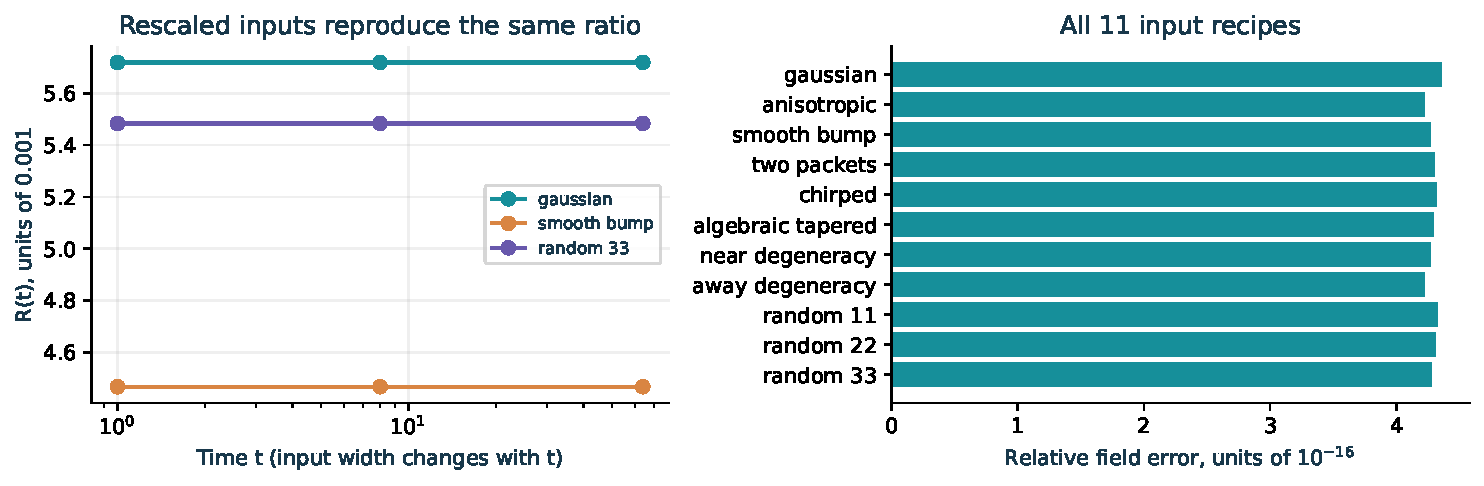
\includegraphics[width=1\linewidth]{visuals/research_scaling.pdf}
\caption{Matched-grid cubic scaling checks for eleven input recipes.}\label{fig:scaling}
\end{figure}

\takeaway{All eleven recipes pass the scaling check. Across 33 evaluations,
the largest relative complex-field discrepancy is \texttt{\ResearchScaleError}.}
The calculation uses $\lambda=1/2,1,2$, hence times $64,8,1$. A length-144,
$96^3$ grid is rescaled to length $144/\lambda$ and spacing $1.5/\lambda$.
Initial data and the dispersion symbol are reevaluated on each scaled grid.
The left panel shows three representative recipes; the right summarizes all eleven.

\textbf{What this verifies.} This is a check of the discrete implementation of an
exact symmetry. The matched grids make the relation exact even for a finite
periodic model; machine-precision agreement is not a new whole-space error bound.


\begin{proposition}[Obstruction to a faster uniform homogeneous rate]
Fix $s\in\{-1,1\}$ and $\beta=0$. Suppose a constant $C$ satisfies
\begin{equation}
\|\,|D_x|^{1/2}S_{s,0}(t)f\|_\infty\le C t^{-\gamma}\|f\|_1
\end{equation}
for every Schwartz function $f$ and every $t\ge1$. Then $\gamma\le7/6$.
\end{proposition}
\noindent\textit{Proof.}
For $f_\lambda(X)=\lambda^3f(\lambda X)$, homogeneity gives
\begin{equation}
|D_x|^{1/2}S_{s,0}(t)f_\lambda(X)
=\lambda^{7/2}\bigl[|D_x|^{1/2}S_{s,0}(\lambda^3t)f\bigr](\lambda X),
\qquad \|f_\lambda\|_1=\|f\|_1.
\end{equation}
Choose $f$ whose Fourier transform is smooth, compactly supported away from
$k_x=0$, and nonzero. The weighted solution at time one then has a finite,
strictly positive supremum $A$. For $0<\lambda\le1$, apply the hypothesized bound
at $t=\lambda^{-3}$ to obtain
\begin{equation}
\lambda^{7/2}A\le C\lambda^{3\gamma}\|f\|_1.
\end{equation}
If $\gamma>7/6$, division by $\lambda^{7/2}$ and passage to $\lambda\to0$
contradict $A>0$.\hfill$\square$

\noindent\textbf{Remark.} This analytical deduction does not prove the upper
bound with exponent $7/6$, determine its optimal constant, or settle fixed-input
asymptotics. The fixed inhomogeneous symbol with $\beta=1$ does not have the same
scaling symmetry.

\subsection{Spectral location and degeneracy}\label{research2}
We vary longitudinal width $\sigma_x\in\{3,6\}$ and spectral offset
$q_x+\beta\in\{-0.75,-0.25,0,0.25,0.75\}$, holding transverse width at 3.
These give twenty cases. Three more target the second curvature-degenerate set,
two impose zero spatial integral, and one supplies a Gaussian cancellation control:
26 inputs, each evaluated at $t=4,8,16$.

\begin{figure}[!htbp]\centering
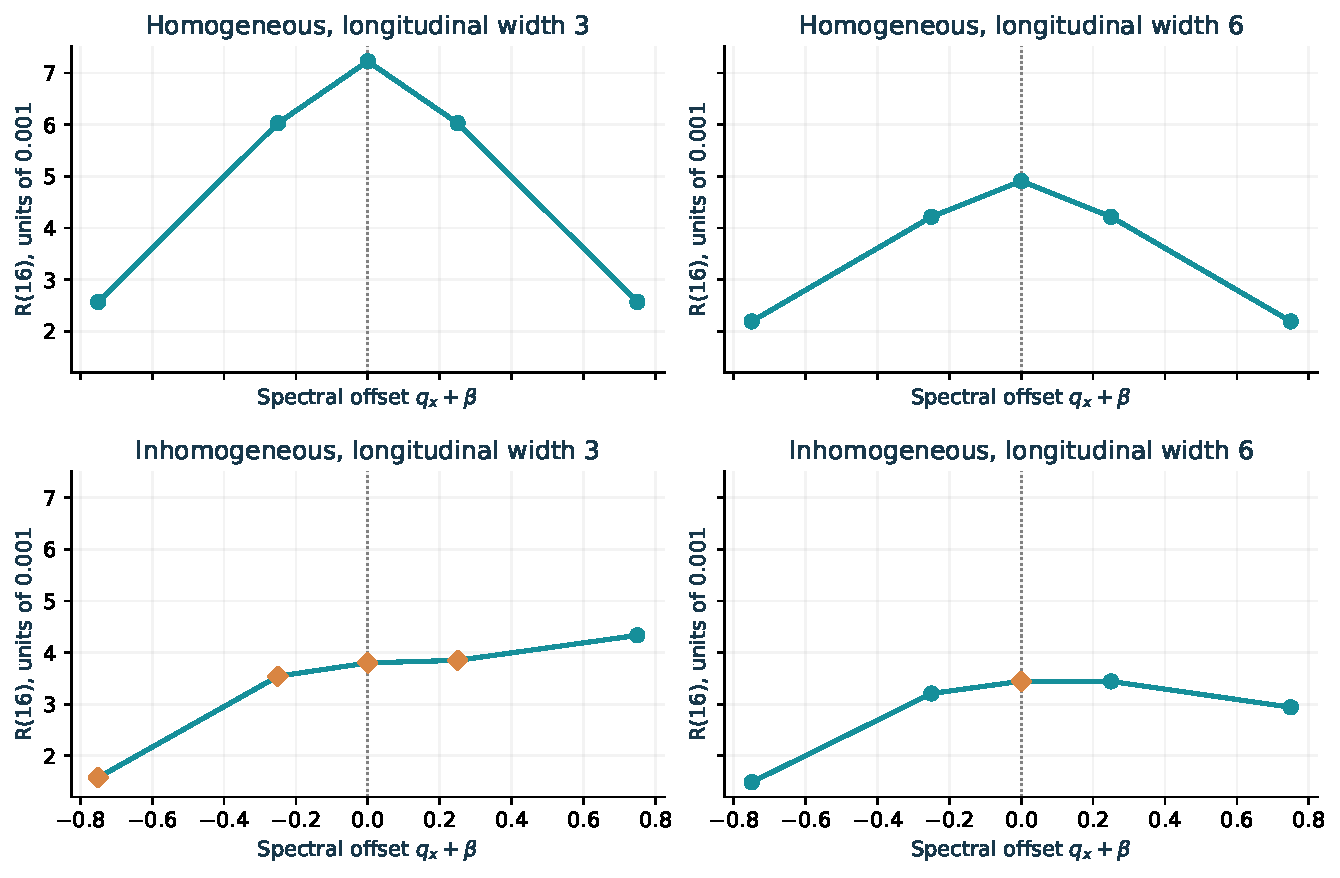
\includegraphics[width=.94\linewidth]{visuals/research_sweep.pdf}
\caption{Dependence of compensated peaks on spectral offset and longitudinal width.}\label{fig:sweep}
\end{figure}

\textbf{Reading the markers.} Circles use the fine 3D FFT result after passing
the 2\% screen. Diamonds use a separate Gaussian-integral follow-up after the
initial screen failed. The dotted line marks the multiplier's cusp.

\takeaway{The homogeneous ratios are largest at the central frequency among
these sampled offsets. The inhomogeneous patterns differ. Frequency location
and width both matter; there is no single ordering that transfers across regimes.}
The original checks compare lengths 144 and 192 at spacing 1.5, then spacings
1.5 and 1 at length 192. \ResearchPass\ of 78 case--time measurements pass the
2\% screen. Eight are flagged and recomputed using analytic transverse integration,
periods 8192 and 16384, radial limits 256 and 512, and local integral optimization. For the odd Gaussian control, the Fourier
amplitude is multiplied by $-i\sqrt{\pi/2}\,\sigma_x k$ to enforce exact continuum
$L^1=1$ normalization; the other follow-ups use normalized Gaussians.
\ResearchFollowPass\ of eight pass the 0.1\% follow-up screen. The largest change
between those two broad searches is \ResearchFollowChange; the largest correction
to an original fine-grid peak is \ResearchCorrection.

\textbf{Second degeneracy.} For the inhomogeneous symbol we also test
$q_x=0.5$, $q_y=\sqrt{0.75}+\delta$ with $\delta=-0.2,0,0.2$ and widths 6.
The middle center lies on $q_x(q_x+1)=q_y^2$. These are localized Gaussian spectra,
not exact support on the surface. All three pass the original screen at $t=16$;
the central case is not the largest of the three. This small test does not identify
a worst-case input.

\subsection{Cancellation and concentration}\label{research3}
For each regime, compare an unshifted Gaussian with
$f(X)\propto x\exp[-|X|^2/18]$, normalized separately to $L^1=1$.
The latter has zero spatial integral by oddness: low-frequency cancellation is
built into the input rather than inferred from a picture.

\begin{figure}[!htbp]\centering
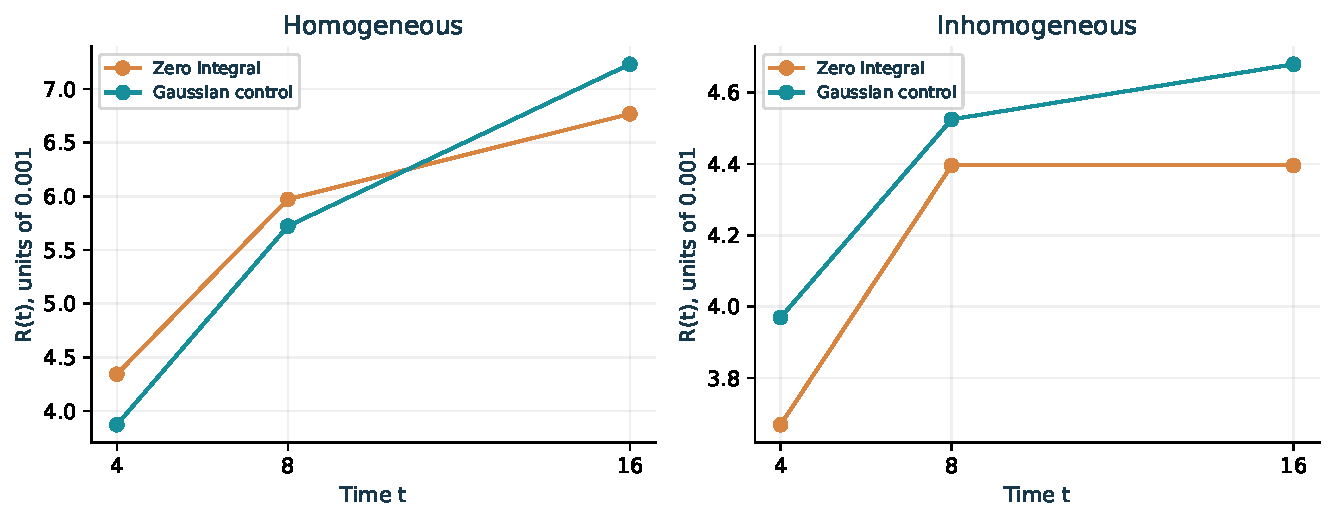
\includegraphics[width=.88\linewidth]{visuals/research_cancellation.pdf}
\caption{Compensated peaks for Gaussian and zero-integral initial data.}\label{fig:cancellation}
\end{figure}

\textbf{Interpretation.} These are short-time ratios, not fitted asymptotic rates.
The inhomogeneous zero-integral ratio is almost flat from $8$ to $16$, within
the numerical differences tested here. A zero integral changes the curve but does not, by itself, establish a stronger
uniform estimate. These inputs still have Gaussian spectral tails; no experiment
with strictly supported spectra away from degeneracies has been completed.

\begin{figure}[!htbp]\centering
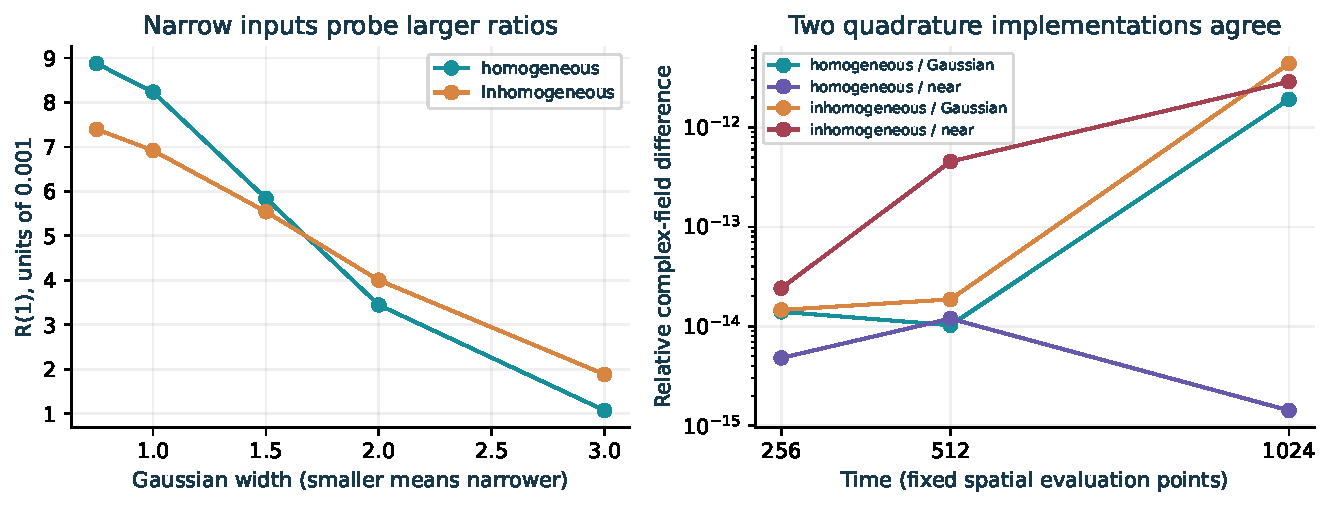
\includegraphics[width=.88\linewidth]{visuals/research_quadrature.pdf}
\caption{Concentration tests at $t=1$ and independent pointwise quadrature comparisons through $t=1024$.}\label{fig:quadrature}
\end{figure}

\textbf{Left: concentrated inputs.} At $t=1$, exactly $L^1$-normalized Gaussian
widths decrease from 3 to 0.75. Ratios increase in both regimes. All ten cases pass
a 2\% numerical screen: longitudinal period/radial extent are doubled, radial
spacing is halved, and candidate peaks are checked by non-periodic integration.
The longitudinal spacing is 0.25 and the narrowest width spans three such steps.

\takeaway{Narrower inputs probe larger ratios here, but five widths do not
establish convergence to a kernel maximum or determine the optimal constant.}
\textbf{Right: independent integration.} The integration comparison is discussed below. Its later-time points evaluate fixed coordinates, not newly located maxima.

\subsection{Independent oscillatory quadrature}\label{research4}
We compare two separately implemented methods for the reduced Gaussian integral.
Both handle the multiplier cusp at $k=-\beta$, but use different panel placement
and integration rules.
\begin{center}\begin{tabular}{p{.26\linewidth}p{.65\linewidth}}\toprule
Method & How it evaluates the integral\\\midrule
Fixed Gauss--Legendre & 64 Gaussian-frequency panels plus a cusp split;
$k=-\beta\pm u^2$ regularization; 256 and 512 nodes per panel.\\
Adaptive Gauss--Kronrod & Panels limit the principal cubic phase variation;
stationary points of $tk^3+xk$ are inserted; the residual complex amplitude is
integrated adaptively after a separately implemented cusp substitution.\\\bottomrule
\end{tabular}\end{center}
\takeaway{Across twelve pointwise comparisons, the maximum relative complex-field
difference is \texttt{\ResearchQuadError}. No adaptive integration warnings were
recorded. Expanding frequency truncation from 12 to 14 Gaussian standard deviations
changes values by at most \texttt{\ResearchQuadTail} relatively.}
For each of the four earlier Gaussian-family cases, we keep its refined $t=256$
peak coordinates and evaluate the field there at $256,512,1024$. The 512-node
Gauss--Legendre values agree with the adaptive calculation. For two cases at
$1024$, changing from 256 to 512 nodes changes the field by about $10^{-7}$
relatively, showing why integration order needs checking as time increases.

\textbf{What has advanced.} We have verified a scaling identity, completed a
controlled frequency sweep with follow-ups for every initially flagged point,
compared cancellation inputs, tested a family of concentrated inputs, and checked
a second integration implementation at later times.

\textbf{What has not advanced yet.} Global peak searches at $512$ and $1024$
have not been performed. Their locations can move, so the pointwise comparisons
cannot extend the decay curves. The new screens remain numerical consistency
checks, not certified bounds on a continuum supremum. No measured fluid data or
full nonlinear water-wave simulation is added in this batch.

\textbf{Research connection.} Frequency targeting is motivated by Ben-Artzi,
Koch and Saut, \href{https://doi.org/10.1081/PDE-120025491}{\emph{Dispersion Estimates
for Third Order Equations in Two Dimensions}} (2003). Stationary-point-aware
integration is motivated by Huybrechs, Kuijlaars and Lejon,
\href{https://arxiv.org/abs/1806.06549}{\emph{A Numerical Method for Oscillatory
Integrals with Coalescing Saddle Points}} (2019), and Gibbs, Hewett and Huybrechs,
\href{https://arxiv.org/abs/2307.07261}{\emph{Numerical evaluation of oscillatory
integrals via automated steepest descent contour deformation}} (2024).
Our adaptive method is a simpler comparison calculation; it does not implement
their published algorithms or claim their error guarantees.

\textbf{Reproduce.} Run \texttt{research\_experiments.py} with arguments
\texttt{scaling}, \texttt{sweep}, \texttt{quadrature}, and \texttt{identity}; then
run \texttt{refine\_research\_flags.py} and \texttt{report/make\_research\_report.py}.
Case-level checkpoints, configurations and summaries are in
\texttt{results/research\_experiments/}. \par The annotated reading note is \texttt{research/literature\_review.md}.

\section{Discussion and further questions}

\subsection{Interpretation of the evidence and proposed continuation}\label{discussion}
\textbf{The numerical conclusion.} The experiments support the reproducibility
of the implemented linear model and the stability of identified peaks under
specified computational changes. They reveal pronounced dependence on initial
spectral center, bandwidth and phase. Those observations are useful for selecting
harder tests; they do not establish a uniform operator bound.

\textbf{Why the current curves are not counterexamples.} The constant in the
claimed estimate is unspecified. An increasing ratio over five time doublings
could still approach a finite limit, and a sampled maximum can be distorted by
spatial truncation. A serious counterexample candidate would need growth that
survives independent refinement and a mathematical argument establishing why it
cannot remain bounded, or a contradiction to an independently established constant.

\textbf{Why faster decay for a subclass remains interesting.} The homogeneous
scaling obstruction applies to an unrestricted $L^1$ formulation. Extra moment
conditions, quantified spectral localization or additional weighted norms change
the class and may change the question. The present cancellation example alone
does not specify or prove such an improved estimate. Its Gaussian spectral tails
also mean it is not supported strictly away from degeneracies.

\begin{center}\begin{tabular}{p{.25\linewidth}p{.65\linewidth}}\toprule
Priority & Proposed next step and criterion\\\midrule
1. Selected cases & Enlarge and refine the exact seed-33 and two-packet weighted
calculations. Require stable full-volume candidate maxima before extending time.\\
2. Later Gaussian times & Perform global searches at $512$ and $1024$; the completed
pointwise quadrature comparison is a prerequisite, not a substitute.\\
3. Restricted input class & Choose a precise cancellation or spectral-support
condition; derive its expected asymptotic behavior before fitting a numerical exponent.\\
4. Kernel sharpness & Continue the normalized concentration sequence with separate
frequency-tail, quadrature and spatial checks; seek evidence of a limiting kernel norm.\\
5. Physical validation & Specify a water-wave envelope model and physical scales,
then reconstruct a surface and compare with suitable measured or Euler data.\\\bottomrule
\end{tabular}\end{center}
\callout{\textbf{Decision for the next work session.} The next work session can choose between extending the
well-checked Gaussian time window and strengthening convergence for the more
visually informative non-Gaussian cases. Both advance the project, but they answer
different questions and should retain separate evidence standards.}

The project archive retains original and refined values separately, including
failed initial screens. This distinction is essential for interpreting changes
in a curve as physical dispersion rather than changes in the computation.

\section{Relation to the literature}

\subsection{Analytical and numerical context}\label{literature}
\textbf{Primary research target.} R. Mosincat, D. Pilod and J.-C. Saut,
\emph{On Third Order Nonlinear Schr\"odinger Equations}, supplied manuscript dated
January 22, 2026. Section 6 gives the three-dimensional canonical estimates under
study. The local supplied version remains our reference; no public replacement
version was verified in the literature search.

\textbf{Cubic dispersion and spectral geometry.} M. Ben-Artzi, H. Koch and
J.-C. Saut (2003), \href{https://doi.org/10.1081/PDE-120025491}{\emph{Dispersion Estimates
for Third Order Equations in Two Dimensions}}, CPDE 28, 1943--1974. Their study of
cubic normal forms and degenerate stationary points motivates deliberately moving
packet spectra across curvature-degenerate sets. It is a two-dimensional methodological
precedent, not a theorem for our three-dimensional weighted operator.

\textbf{Nonlinear Dysthe theory.} R. Mosincat, D. Pilod and J.-C. Saut (2021),
\href{https://arxiv.org/abs/2007.01613}{\emph{Global well-posedness and scattering for
the Dysthe equation in $L^2(\mathbb R^2)$}}, JMPA 149, 73--97. Small-data scattering
places the linear estimates in a nonlinear context. The regularity sharpness in
that work is distinct from sharpness of the decay exponent studied here.
R. Grande, K. M. Kurianski and G. Staffilani (2021),
\href{https://arxiv.org/abs/2006.13392}{\emph{On the nonlinear Dysthe equation}},
Nonlinear Analysis 207, 112292, develops anisotropic estimates relevant to the
importance of direction and frequency localization.

\textbf{Oscillatory integration.} S. Olver (2007),
\href{https://www.cambridge.org/core/journals/european-journal-of-applied-mathematics/article/abs/momentfree-numerical-approximation-of-highly-oscillatory-integrals-with-stationary-points/0E02A1874E775BB219E5A2CE2DC0221B}{\emph{Moment-free numerical approximation of highly oscillatory integrals with stationary points}},
provides an early stationary-point-aware approach; our assessment used the publisher abstract.
D. Huybrechs, A. B. J. Kuijlaars and N. Lejon (2019),
\href{https://arxiv.org/abs/1806.06549}{\emph{A Numerical Method for Oscillatory Integrals
with Coalescing Saddle Points}}, and A. Gibbs, D. P. Hewett and D. Huybrechs (2024),
\href{https://arxiv.org/abs/2307.07261}{\emph{Numerical evaluation of oscillatory integrals
via automated steepest descent contour deformation}}, JCP 501, 112787, motivate
more robust independent quadrature. Our phase-partitioned adaptive method is not
an implementation of their algorithms and does not inherit their guarantees.

\textbf{Physical surface reconstruction.} P. Guyenne, A. Kairzhan and C. Sulem
(2022), \href{https://doi.org/10.1137/21M1432788}{\emph{Hamiltonian Dysthe Equation for
Three-Dimensional Deep-Water Gravity Waves}}, MMS 20, 349--378, develops a refined
free-surface reconstruction and comparisons with Euler simulations. Here the
fluid domain is three-dimensional but the surface has two horizontal coordinates.
It supplies a route to physical validation, not validation of our current optical
or canonical snapshots.

\textbf{Access and scope.} These references were checked against author papers,
preprints and publisher records on September 9, 2026. The fuller annotated note
and the scaling derivation are included in \path{research/literature_review.md}.
The review is targeted rather than exhaustive.


The cited analytical background comprises~\cite{BAKS,MPS2021,GKS}; numerical
integration references are~\cite{Olver,HKL,GHH}. Physical interpretation is
informed by~\cite{GKSfluid,Salmon}. These works supply context and motivation,
not validation of the present finite computational searches.
\clearpage\begin{thebibliography}{9}
\bibitem{MPSdraft} R. Mosincat, D. Pilod and J.-C. Saut,
\emph{On Third Order Nonlinear Schr\"odinger Equations}, supplied manuscript,
January 22, 2026, Section 6.
\bibitem{BAKS} M. Ben-Artzi, H. Koch and J.-C. Saut,
Dispersion estimates for third order equations in two dimensions,
\emph{Comm. Partial Differential Equations} 28 (2003), 1943--1974.
\href{https://doi.org/10.1081/PDE-120025491}{doi:10.1081/PDE-120025491}.
\bibitem{MPS2021} R. Mosincat, D. Pilod and J.-C. Saut,
Global well-posedness and scattering for the Dysthe equation in $L^2(\mathbb R^2)$,
\emph{J. Math. Pures Appl.} 149 (2021), 73--97.
\href{https://arxiv.org/abs/2007.01613}{arXiv:2007.01613}.
\bibitem{GKS} R. Grande, K. M. Kurianski and G. Staffilani,
On the nonlinear Dysthe equation, \emph{Nonlinear Analysis} 207 (2021), 112292.
\href{https://arxiv.org/abs/2006.13392}{arXiv:2006.13392}.
\bibitem{Olver} S. Olver, Moment-free numerical approximation of highly oscillatory
integrals with stationary points, \emph{European J. Appl. Math.} (2007).
Assessment limited to the publisher abstract.
\bibitem{HKL} D. Huybrechs, A. B. J. Kuijlaars and N. Lejon,
A numerical method for oscillatory integrals with coalescing saddle points,
\emph{SIAM J. Numer. Anal.} (2019).
\href{https://arxiv.org/abs/1806.06549}{arXiv:1806.06549}.
\bibitem{GHH} A. Gibbs, D. P. Hewett and D. Huybrechs,
Numerical evaluation of oscillatory integrals via automated steepest descent
contour deformation, \emph{J. Comput. Phys.} 501 (2024), 112787.
\href{https://arxiv.org/abs/2307.07261}{arXiv:2307.07261}.
\bibitem{GKSfluid} P. Guyenne, A. Kairzhan and C. Sulem,
Hamiltonian Dysthe equation for three-dimensional deep-water gravity waves,
\emph{Multiscale Model. Simul.} 20 (2022), 349--378.
\href{https://doi.org/10.1137/21M1432788}{doi:10.1137/21M1432788}.
\bibitem{Salmon} R. Salmon, \emph{Introduction to Ocean Waves}, Chapter 2,
pp. 25--26, \href{https://www-pord.ucsd.edu/rsalmon/111.textbook.pdf}{online text}.
\end{thebibliography}
\clearpage\appendix

\section{Optical baseline and verification}

\subsection{Equation and numerical method}\label{optical}
We solve
\begin{equation}
 iE_t+(1-i\varepsilon_1\partial_z)\Delta_\perp E-E_{zz}
       -i\varepsilon_2 E_{zzz}=0,
 \qquad \Delta_\perp=\partial_x^2+\partial_y^2.
 \label{eq:pde}
\end{equation}
With $\widehat E(\mathbf k)=\int E(\mathbf x)e^{-i\mathbf k\cdot\mathbf x}\,d\mathbf x$,
\begin{equation}
 \widehat E(\mathbf k,t)=e^{-it\omega(\mathbf k)}\widehat E_0(\mathbf k),\qquad
 \omega=(1+\varepsilon_1 k_z)(k_x^2+k_y^2)-k_z^2+\varepsilon_2k_z^3.
 \label{eq:prop}
\end{equation}
This matches the paper's symbol (6.6). Its equation (1.32) prints the opposite sign
on the mixed third derivative. We follow (1.27) and (6.6) consistently; this choice
must be retained when comparing with another implementation.

An FFT computes the initial coefficients once. For each requested $t$, we multiply
by the phase in \eqref{eq:prop} and perform an inverse FFT. Evolution of the retained
modes is exact up to floating-point arithmetic. There is no time-marching truncation
error; spatial sampling, finite-box effects, and sampling the peak remain relevant.
At a fixed total grid size $N$, $M$ snapshots cost $O(MN\log N)$.

\begin{center}
\begin{tabular}{ll}\toprule
Setting & Value \\\midrule
Computational box & $[-48,48)^3$, periodic \\
Production grid & $96^3$ points; $\Delta x=\Delta y=\Delta z=1$ \\
Arithmetic & Torch CPU, complex128, four threads \\
Evolution times & 25 snapshots, $t=0,0.25,\ldots,6$ \\
Parameters & $\varepsilon_1=1$; $\varepsilon_2\in\{1,-1/3,0\}$ \\
Initial Gaussian & $E_0=e^{-(x^2+y^2+z^2)/18}e^{i\mathbf q\cdot\mathbf x}$ \\
Frequency shifts & $\mathbf q=0$, $(\pi/6,0,0)$, $(0,0,\pi/6)$ \\\bottomrule
\end{tabular}
\end{center}
The shift is eight Fourier bins on the production box. All three initial magnitudes
are identical, with peak one. Positive $\varepsilon_2$ and $-\varepsilon_1/3$ connect
to the parameter cases in Theorem 5.1; the zero case is included as a linear comparison,
without extending that nonlinear theorem to it. All quantities are dimensionless.

\subsection{Peak evolution and parameter dependence}\label{optical11}
The peak curves below are spatial grid maxima, not amplitudes at a fixed point.
All three parameter families spread over the observation window. The response to
a $z$-shift depends strongly on $\varepsilon_2$, even though the initial magnitudes
and norms are unchanged.

\begin{figure}[!htbp]\centering
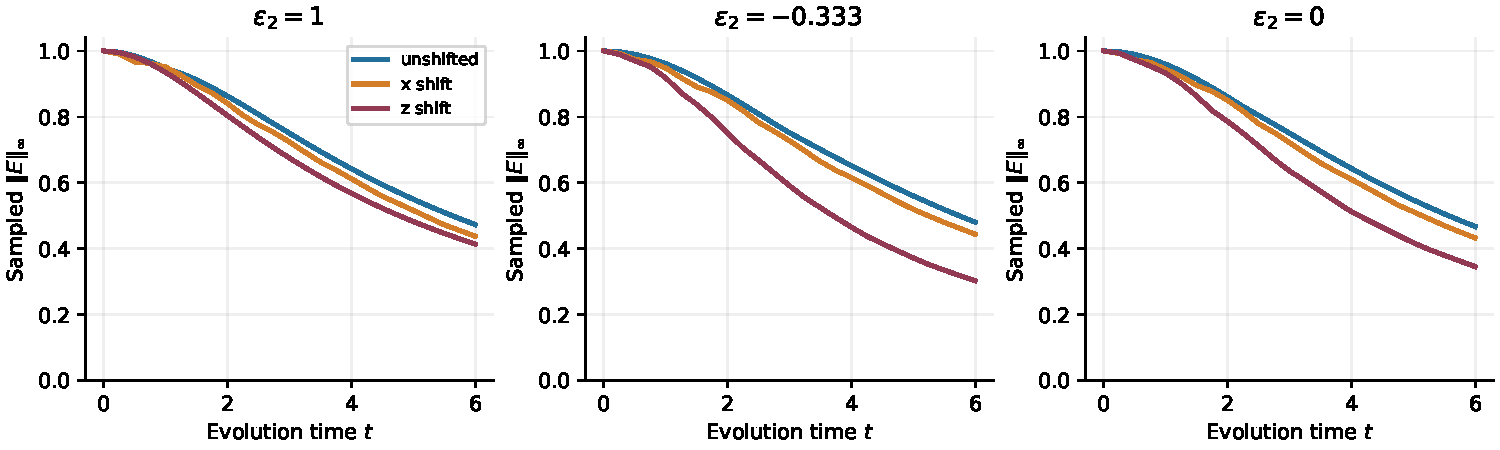
\includegraphics[width=1\linewidth]{figures/peak_decay.pdf}
\caption{Optical baseline: sampled peak magnitudes for the parameter and modulation cases.}\label{fig:opticalpeaks}
\end{figure}

Sampled $L^\infty$ histories. Lines join directly evaluated
snapshots; they do not represent a numerical time integrator.

\begin{center}
\begin{tabular}{llrrrr}\toprule
$\varepsilon_2$ & Initial spectrum & Peak at $t=6$ & $s_x$ & $s_y$ & $s_z$ \\\midrule
\FinalRows
\bottomrule\end{tabular}
\end{center}
Here $s_j$ is the standard deviation of coordinate $j$ under the normalized intensity
$|E|^2/\int|E|^2$. Initially $s_x=s_y=s_z=3/\sqrt2\simeq2.121$.
Widths describe the packet as a whole and remain meaningful when its maximum moves.

For $\varepsilon_2=1$, the final peaks are approximately $0.473$ (unshifted),
$0.438$ ($x$-shift), and $0.414$ ($z$-shift). For $\varepsilon_2=-1/3$, the
$z$-shifted peak is approximately $0.303$. The $z$-shift therefore need not have
the same effect across dispersion parameters.

\textbf{What these curves establish.} They demonstrate finite-time spreading and
directional sensitivity for these initial data. They do not establish an asymptotic
decay exponent, monotone decay for arbitrary data, or a universal decay constant.
The reported $L^2$ norm is constant to relative error \MassError; this is
dispersion without imposed damping.

\subsection{Spatial slices}\label{optical12}

\begin{figure}[!htbp]\centering
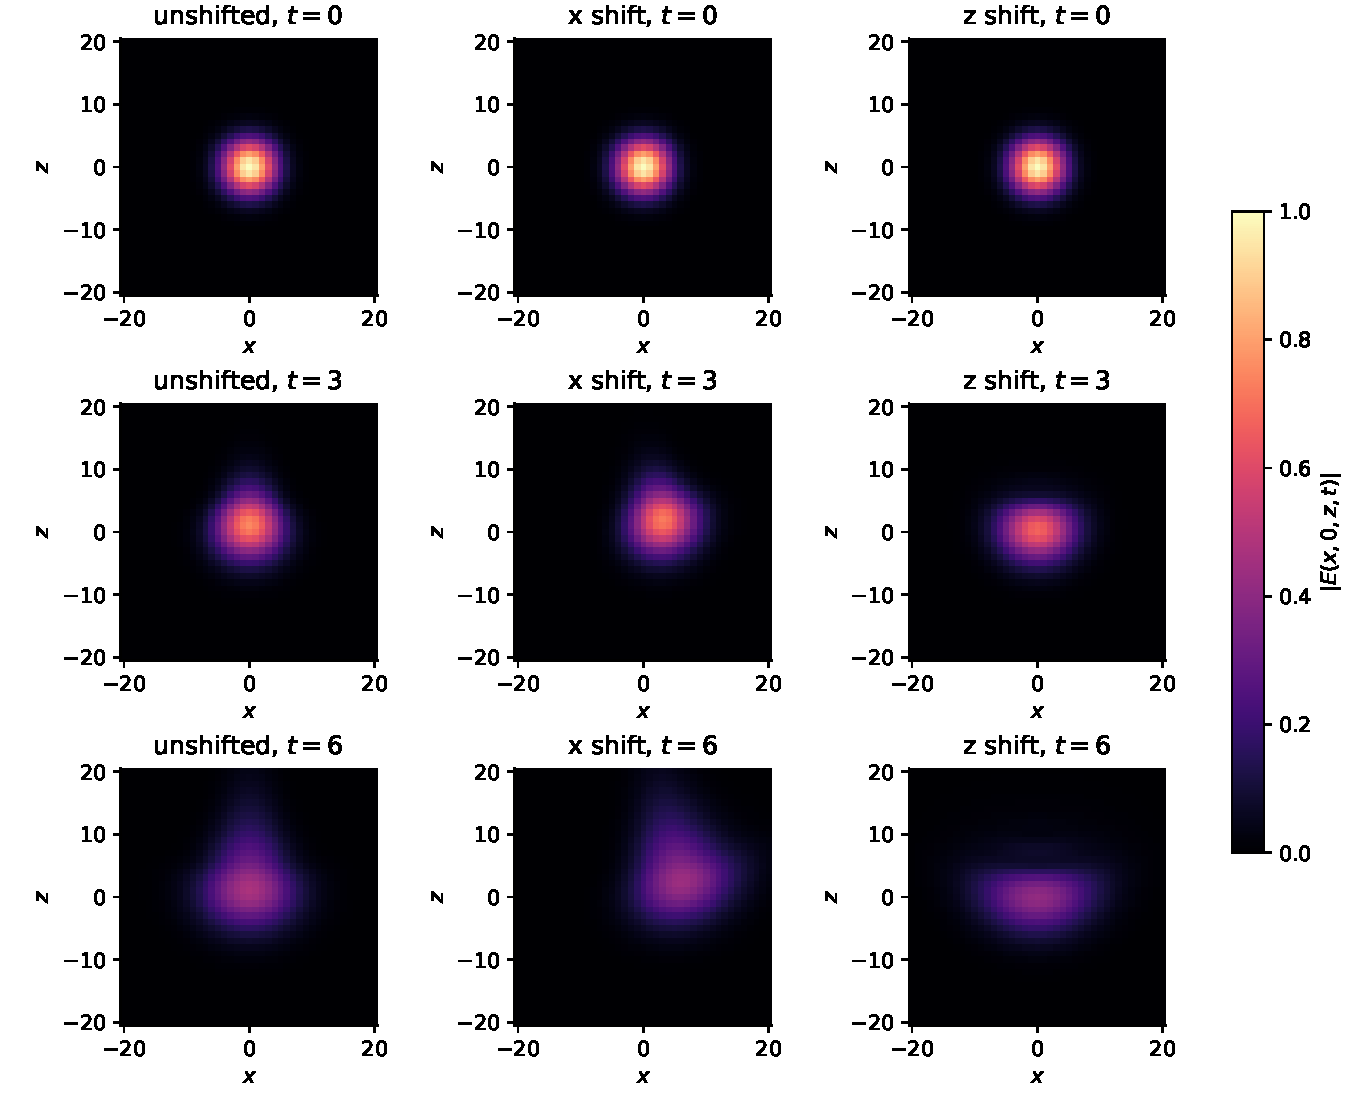
\includegraphics[width=.97\linewidth]{figures/slices.pdf}
\caption{Optical baseline: $y=0$ magnitude slices for $\varepsilon_2=1$.}\label{fig:opticalslices}
\end{figure}

Magnitude on the $y=0$ plane for $\varepsilon_2=1$. Columns
compare unshifted, $x$-shifted, and $z$-shifted initial spectra. Rows show
$t=0,3,6$. Every panel uses the same color range, making the loss of peak
amplitude visible. The displayed window is $[-20,20]^2$ within the larger
computational box; the color plots are slices of genuine three-coordinate solutions.

Modulation changes propagation as well as deformation. A slice alone can miss
an off-plane maximum, which is why Figure~\ref{fig:opticalpeaks} and the table use the full volume.
Full complex fields at $t=6$ are saved in the project snapshot archive and can be regenerated from the included solver.

\subsection{Directional spreading and generic initial data}\label{optical13}

\begin{figure}[!htbp]\centering
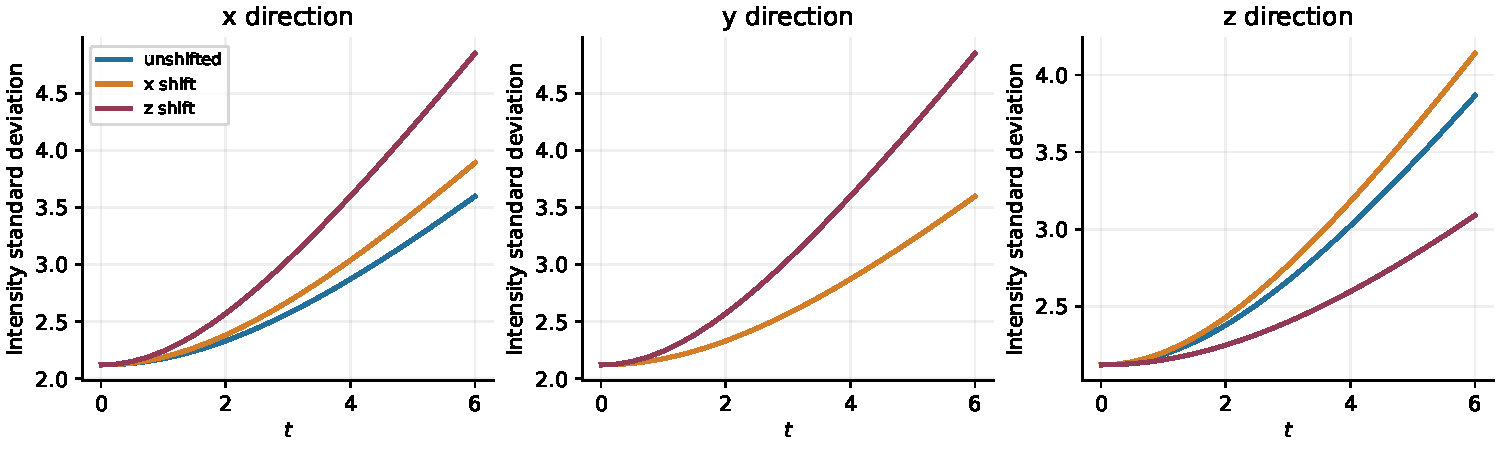
\includegraphics[width=1\linewidth]{figures/widths.pdf}
\caption{Optical baseline: intensity widths in the three coordinate directions.}\label{fig:widths}
\end{figure}

Intensity widths for $\varepsilon_2=1$. An $x$-shift breaks
the equality of the transverse widths; a $z$-shift changes both transverse widths
together. Exchanging $x$ and $y$ in the shifted experiment agrees to maximum
absolute field error \SymmetryError.

This behavior is consistent with the group velocity of \eqref{eq:prop}:
\begin{equation}
 \nabla_{\mathbf k}\omega=
 \bigl(2(1+\varepsilon_1k_z)k_x,\;
       2(1+\varepsilon_1k_z)k_y,\;
       \varepsilon_1(k_x^2+k_y^2)-2k_z+3\varepsilon_2k_z^2\bigr).
\end{equation}
Changing $k_z$ changes the transverse dispersion factor itself. Changing $k_x$
also affects longitudinal transport through the $k_x^2$ term. The axes are coupled.


\begin{figure}[!htbp]\centering
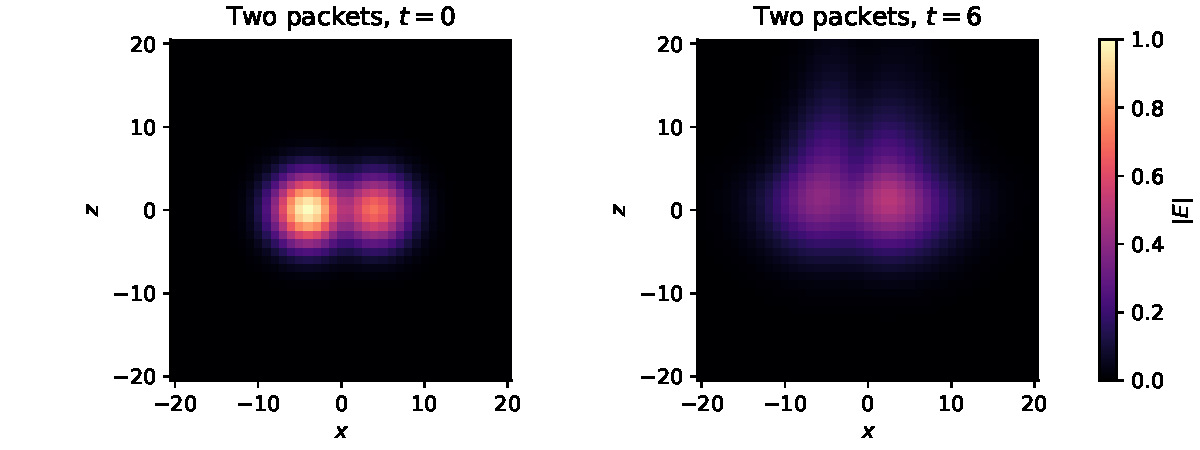
\includegraphics[width=.85\linewidth]{figures/generic.pdf}
\caption{Optical baseline: a non-Gaussian two-packet initial profile and its propagated magnitude.}\label{fig:generic}
\end{figure}

A non-Gaussian initial profile, propagated with the same solver:
\begin{equation}
 E_0=e^{-((x+4)^2+y^2+z^2)/18}
       +0.7i\,e^{-((x-4)^2+y^2+z^2)/18},\qquad \varepsilon_2=1.
\end{equation}
This example demonstrates that the solver accepts a sampled complex field without
requiring a Gaussian formula. Its separate convergence study is not included here.

\setlength{\parskip}{4pt}
\subsection{Verification and interpretation limits}\label{optical14}
\textbf{Algebraic checks.} A periodic plane wave with wavevector $(1,2,-1)$ at
$\varepsilon_1=\varepsilon_2=1$ has $\omega=-2$, hence exact multiplier $e^{2it}$.
The solver agrees at $t=0.73$ to \PlaneError\ in maximum error. Forward/backward
propagation of the $z$-shifted packet gives relative $L^2$ error \ReverseError.
These checks complement conservation, which alone cannot detect a wrong phase sign.

\textbf{Grid refinement.} The table compares the $z$-shifted field at $t=6$ against
a $192^3$ computation on the same length-96 box. The reference is restricted to
the coarse nodes before measuring relative discrete $L^2$ error.
\begin{center}\begin{tabular}{rrrr}\toprule
Grid & $\varepsilon_2=1$ & $\varepsilon_2=-1/3$ & $\varepsilon_2=0$ \\\midrule
\GridRows
\bottomrule\end{tabular}\end{center}
This demonstrates convergence of sampled fields on a fixed periodic box. It does
not imply that a grid maximum equals the continuum supremum. Across all nine final
Gaussian fields, doubling the resolution changes the sampled peak by at most
\PeakPercent\ percent. Figure~\ref{fig:opticalpeaks} retains the production-grid maxima.

\textbf{Domain enlargement.} At spacing $0.5$, length-48 and length-72 boxes are
compared to length 96 on the common cube $[-24,24)^3$, using the $z$-shifted field.
A separate check compares each production field to a length-144 box at spacing 1,
restricted to the entire original box. The last column is the worst of all three shifts.
\begin{center}\begin{tabular}{rrrr}\toprule
$\varepsilon_2$ & $L=48$ vs. 96 & $L=72$ vs. 96 & $L=96$ vs. 144 \\\midrule
\DomainRows
\bottomrule\end{tabular}\end{center}
Values are relative discrete $L^2$ differences on the stated comparison regions.
The agreement improves on enlarging the box, but it is evidence on $0\le t\le6$,
not permission to extrapolate indefinitely on a periodic domain.

\textbf{Independent whole-space check.} For the Gaussian, the transverse Fourier
integrals can be evaluated analytically, leaving a one-dimensional adaptive integral
in $k_z$. At $t=6$, we compare the origin, $(3,-2,5)$, and the production peak node
for each of the nine cases. The largest absolute complex-field discrepancy is
\QuadError. Quadrature uses $k_z\in[-5,5]$ with absolute and relative tolerance
$10^{-12}$; Gaussian tails outside this interval are negligible at this precision.
This checks 27 points, not the entire continuum field.

\textbf{Relation to the paper.} Propositions 6.2--6.3 bound a fractional-derivative-weighted
solution in transformed coordinates for $0<\alpha<1$. They do not directly assert
the plotted unweighted peak follows $t^{-(3+\alpha)/3}$. No exponent is fitted here,
and no theorem constant is inferred. The weighted experiments earlier in this report address that separate diagnostic.

\textbf{Reproduction.} From the project folder, run the following commands:
\begin{quote}\small\ttfamily
python3 numerical\_solutions.py\\
python3 report/make\_tables.py
\end{quote}
Compile \texttt{formal\_report.tex} from \texttt{report/}. Dependencies are NumPy, SciPy, Matplotlib, and Torch.
The supplied CSV contains all 225 Gaussian norm records; JSON contains checks and
configuration; the NPZ contains nine final Gaussian fields and the two-packet field.
The recorded computation and figure-generation time was \Runtime\ seconds on this
host; this is one CPU run, not a hardware benchmark or a GPU measurement.

\textbf{Source.} R. Mosincat, D. Pilod, and J.-C. Saut,
\emph{On Third Order Nonlinear Schr\"odinger Equations}, supplied manuscript
\texttt{Dysthe3D-2.pdf}, pp. 9--10 and 18--23. No publication status is assumed.

\section{Canonical numerical methods and audits}

\subsection{Intermediate-time Fourier computations}\label{intermediate}
We use $S(t)f=\mathcal F^{-1}(e^{itw}\widehat f)$ with
\begin{equation}w=k_x^3+3s k_x(k_y^2+k_z^2)+3\beta(k_y^2+k_z^2),\end{equation}
where $(s,\beta)=(-1,0)$ or $(1,1)$. This follows the proofs of Propositions
6.2--6.3; the signs printed in (6.1) are inconsistent. The weighted multiplier is
$|k_x+\beta|^{1/2}$. These are canonical coordinates, not a numerical conversion
of the optical baseline above.

We extend four families in both regimes to $t=16$, four times the first batch's
maximum time. Gaussian is the reference, the compact bump has a broader spectrum,
the near-degeneracy packet targets the multiplier's cusp, and seed 33 represents
the random collection. This is a targeted follow-up, not an exhaustive data search.

Domain checks compare lengths 96, 192, and 288 at spacing 1. A separate length-192
grid with spacing $2/3$ checks resolution. Every comparison uses the same continuum
recipe, normalized using its own grid quadrature. The table gives results at $t=16$;
machine-readable files also include $t=4,8$ and complex-field errors on a common cube.

\begin{center}\small
\begin{tabular}{llrrr}\toprule
Equation & Input & $R(16)$ & Domain peak change & Grid peak change\\\midrule
\RefinedRows
\bottomrule\end{tabular}
\end{center}
Domain peak change compares lengths 192 and 288; grid peak change compares
spacings 1 and $2/3$ at length 192. Peak comparisons use each grid's full sampled
maximum, not a fixed spatial point. The plotted length-288 field is not itself
also refined to spacing $2/3$, so the checks do not establish joint convergence.

\textbf{Observed behavior.} \ObservedResult

\textbf{Numerical qualification.} \CheckResult
The fractional multiplier can produce long spatial tails, and errors can vary
nonmonotonically with box size near its cusp. A field's relative $L^2$ difference
and its maximum-amplitude difference are distinct: this follow-up prioritizes the
maximum because it appears in the inequality, while retaining both diagnostics.

\textbf{Inference.} These experiments do not establish a faster universal decay
rate, a theorem constant, or a counterexample. A convincing candidate violation
would require a controlled sequence of times or normalized inputs with increasing
ratios that survives numerical refinement. A short transient slope is insufficient.
Cases that fail the peak checks should be refined before being interpreted as
evidence about the whole-space bound.

\textbf{Data and reproducibility.} Run \texttt{python3 decay\_dataset.py}, then
\texttt{python3 refine\_decay.py}. Results are in
\texttt{results/decay\_dataset/}: \texttt{refined\_decay.csv},
\texttt{refinement\_checks.json}, \texttt{REFINEMENT.md}, and the plotted figures.
The first batch's inputs remain available as complex-valued NPZ arrays.
These are artificial inputs. CDIP buoy observations have been identified as a
possible source, but are not imported or presented as three-dimensional measurements.

\textbf{Source.} R. Mosincat, D. Pilod, and J.-C. Saut,
\emph{On Third Order Nonlinear Schr\"odinger Equations}, supplied manuscript
\texttt{Dysthe3D-2.pdf}, Section 6. This supplement follows the stated estimates
as research targets, without claiming to resolve the manuscript's proof details.

\textbf{Visual gallery reproduction.} Run \texttt{python3 report/make\_visual\_gallery.py}.
The script records seeds, grid, normalization, peak values and $L^2$ norms in
\texttt{report/visuals/gallery\_manifest.json}. Rebuild this combined source with
\texttt{python3 report/build\_formal\_report.py}, then compile \texttt{formal\_report.tex}.

\subsection{Gaussian reduction and long-time searches}\label{longmethods}
Let $r=\sqrt{y^2+z^2}$ and use the exactly $L^1$-normalized initial profile
\begin{equation}
 f(x,r)=\frac{\exp[-x^2/(2\sigma_x^2)-r^2/(2\sigma_y^2)]e^{iqx}}
 {(2\pi)^{3/2}\sigma_x\sigma_y^2}.
\end{equation}
The Gaussian has $(\sigma_x,\sigma_y,q)=(3,3,0)$; the near-degeneracy packet
has $(6,3,-\beta)$. Analytically integrating both transverse Fourier variables
reduces the weighted field to
\begin{equation}
 W(x,r,t)=\frac1{4\pi^2}\int_{\mathbb R}
 \frac{|k+\beta|^{1/2}}{d(k,t)}
 \exp\!\left[-\frac{\sigma_x^2(k-q)^2}{2}+i(tk^3+kx)
             -\frac{r^2}{2d(k,t)}\right]dk,
 \qquad d(k,t)=\sigma_y^2-6it(sk+\beta).
\end{equation}
This is the same three-coordinate linear solution for these inputs. Only the
evaluation method changes. The transverse directions are treated on the whole
space; a longitudinal FFT quadrature evaluates many $x$ locations efficiently.
Radial symmetry reduces the spatial peak search to $(x,r)$.

\begin{center}\begin{tabular}{lrrrr}\toprule
Check & $x$ period & $\Delta x$ & Max. $r$ & $\Delta r$\\\midrule
Base & 4096 & 0.5 & 512 & 4\\
Expanded & 8192 & 0.5 & 1024 & 4\\
Refined & 8192 & 0.25 & 1024 & 2\\
Extra expansion at $t=256$ & 32768 & 0.25 & 2048 & 2\\\bottomrule
\end{tabular}\end{center}
The full $(x,r)$ search is followed by local optimization of the peak. At $256$,
the extra expansion changes the sampled peak by at most \LongDomain. An independent
adaptive quadrature of the integral above agrees with the complex field at each
final candidate peak to within \LongQuad\ relative error. The largest sampled
search-boundary amplitude is \LongEdge\ of its case's peak. These checks are
numerical evidence, not a certification that no larger unsampled peak exists.

\textbf{Why the previous box was inadequate.} At $t=256$, the inhomogeneous
near-degeneracy maximum lies around $x=-841$. It would be outside even the
length-288 box used for the earlier $t\le16$ runs. Extending time without changing
the spatial computation would therefore be unreliable.

\textbf{Remaining limits.} The Gaussian-specific reduction cannot be applied
unchanged to arbitrary measured fields or every artificial recipe. The adaptive
quadrature checks selected peak locations; the global search remains finite and
sampled. The two-dimensional radial search, local optimizer status, boundary ratios,
and domain/resolution comparisons are all recorded to make these limits reviewable.

\textbf{Reproduce.} Run \texttt{python3 long\_time\_decay.py}, followed by
\path{python3 report/make_long_time_tables.py}. Results and the graph are under
\texttt{results/long\_time/}; compile \texttt{formal\_report.tex} for this
combined numerical study. Source: the same manuscript, canonical symbols (6.2) and
weighted estimates in Propositions 6.2--6.3.

\subsection{Detailed spatial audit at $t=256$}\label{spatialaudit}
\textbf{Purpose.} Hold time, input, and $\alpha=1/2$ fixed, and vary the spatial
computation. This audit separates longitudinal enlargement from transverse
enlargement. It tests whether the four reported candidate maxima stabilize to
an exploratory relative tolerance of $0.1\%$.

The longitudinal period increases from 32,768 to 65,536 while the radial limit
stays at 2,048. We then search the additional annulus out to radius 4,096.
Finally, we double the longitudinal period again to 131,072, retaining the
larger radial limit. Every broad scan keeps $\Delta x=0.25$ and $\Delta r=2$.
The baseline is the saved final scan from the preceding experiment.

\begin{center}\small
\begin{tabular}{llrrrr}\toprule
Equation & Input & First $L$ change & Radius change & Second $L$ change & Integral check\\\midrule
\SpatialRows
\bottomrule\end{tabular}\end{center}
The three domain columns compare sampled peak magnitudes before and after the
stated expansion. The integral check compares the final Fourier-quadrature field
to an independently evaluated non-periodic integral at the refined candidate peak.
Percentages use the newer or independent result as the denominator. Values are rounded.

\textbf{Result.} \SpatialPassed\ of four cases pass the $0.1\%$ peak screen.
This includes the two longitudinal expansions, the transverse expansion, the
final locally optimized peak drift, and the independent integral check.
The largest change in locally optimized peak magnitude between the final two
periods is \SpatialPeakDrift.

\begin{center}\small
\begin{tabular}{llrrrr}\toprule
Equation & Input & Refined $R(256)$ & $x$ & $r$ & Location drift\\\midrule
\SpatialLocations
\bottomrule\end{tabular}\end{center}
Locations are continuous-coordinate candidate maxima from the independent
integral optimization. The drift is the Euclidean distance in $(x,r)$ between
local peak optimizations at the final two longitudinal periods. Its maximum is
\SpatialLocationDrift. Axial symmetry means a nonzero $r$ represents a ring of
equivalent points, not a unique three-dimensional location.

\textbf{Additional checks.} Local optimization starts from the broad search's
largest sample and refines both $x$ and $r$. Increasing the independent
integral's Gauss--Legendre order from 256 to 512 per panel changes the complex field by
at most \SpatialQuadTighten\ relative to the tighter result. Its integration
interval is split at the fractional multiplier cusp and into 64 Gaussian-frequency
panels. On each side, $k=-\beta\pm u^2$ removes the square-root cusp from the
integration variable. Fixed-order quadrature with an order-doubling check replaces
adaptive quadrature, which issued convergence warnings during local searches.
The largest sampled search-boundary amplitude is \SpatialBoundary\ of
the corresponding peak. Optimizer status and all intermediate measurements are
saved in the per-case JSON records.

\textbf{What we can now say.} At this time and for these four inputs, the peak
values have stronger numerical support from separate domain enlargements,
continuous local refinement, stable locations, and independent integration.
This improves confidence in the reported decay ratios. It does not prove the
maximum is global over all of $\mathbb R^3$, establish an asymptotic decay rate,
or extend reliability to other inputs, values of $\alpha$, or later times.

\textbf{Remaining spatial limitation.} The broad radial mesh is still spaced by
2; refinement is local to the identified maximum, not a global halving of every
cell. A missed narrow peak or a remote maximum is not excluded by these checks.
The report therefore claims numerical spatial stability of the identified peaks,
not a certified supremum.

\textbf{Reproduce.} Run \texttt{python3 spatial\_reliability.py}, then
\texttt{python3 report/make\_spatial\_tables.py}. Results, configurations, and
checkpoints are under \texttt{results/spatial\_reliability/}.

\subsection{Selected-case computation}\label{selectedmethods}
\textbf{Evolution.} We work directly in the homogeneous canonical coordinates of
the supplied manuscript, with
\begin{equation}
 \widehat u(k,t)=e^{itw(k)}\widehat f(k),\qquad
 w(k)=k_x^3-3k_x(k_y^2+k_z^2).
\end{equation}
Equivalently, $u_t+u_{xxx}-3u_{xyy}-3u_{xzz}=0$. The Fourier convention is
$\widehat f(k)=\int f(X)e^{-ik\cdot X}\,dX$. This is the linear propagator used
in the homogeneous weighted estimate; it is not the full nonlinear Dysthe equation.

\begin{center}\begin{tabular}{ll}\toprule
Setting & Value\\\midrule
Computational domain & Periodic cube $[-72,72)^3$\\
Grid & $192^3$, spacing $0.75$\\
Displayed region & $[-24,24]^3$; slices at $y=0$\\
Snapshot times & $0,4,8$\\
Supplementary time series & $0,0.5,\ldots,8$\\
Arithmetic & Torch CPU, complex128\\
Initial normalization & Discrete $L^1=1$ for each input\\
Time evolution & Exact Fourier phase for retained modes\\\bottomrule
\end{tabular}\end{center}
\textbf{Checks and their limits.} The new diagnostic series reproduces the three
selected snapshot times. Integrated squared magnitude is conserved to numerical
precision: the relative $L^2$ changes are below $10^{-11}$. Conservation checks
consistency but cannot establish an accurate whole-space maximum or detect every
phase error. No separate domain enlargement or mesh refinement was performed for
this selected-packet series.

At $t=8$, the maximum sampled amplitude on the displayed cube's boundary is
approximately 16.4\% of the full peak for seed 33 and 6.0\% for the two-packet case.
Thus the 30\% surfaces do not touch that sampled boundary, but weaker tails are
cropped from view. This is a display check, not a test of the computational boundary.
The strong $t=256$ audit in the larger project applies to other Gaussian-based
inputs and must not be transferred to these two cases.

\begingroup\raggedright\textbf{Reproduction.} Run \path{make_figure_review.py} for the selected figures.
Run \path{report/selected_packet_diagnostics.py} for Figure~\ref{fig:diagnostics}, its table, and the
JSON records in \path{results/selected_packets/}. Compile
\path{formal_report.tex} to rebuild this report.\par\endgroup

\section{Checkpoint record and reproducibility}

\subsection{Progression of the investigation}\label{checkpoint}
This checkpoint records the work completed by September 10, 2026. It preserves the
full research narrative and adds a progress record for reviewing and resuming the
project. Preparing this checkpoint adds documentation, not new simulation results.

\textbf{Starting point: a numerical model.} We began with the supplied manuscript
and implemented a three-coordinate linear dispersive model. The optical baseline
established exact Fourier propagation and checks against special solutions,
independent integration, and changes in the spatial grid and box.

\textbf{Making the solution understandable.} We distinguished the complex envelope,
its magnitude, intensity, carrier oscillations, and illustrative water elevation.
Three-dimensional magnitude surfaces and planar slices made the simulated fields
visible. The fluid illustration explains the envelope idea; it is not a calibrated
reconstruction of the canonical three-coordinate solution.

\textbf{Refocusing on the research question.} The investigation moved from visual
spreading to the manuscript's weighted decay estimate. The compensated ratio
$R(t;f)$ became the central observable. Gaussian data supplied a starting point,
then eleven artificial input recipes broadened the tests to phases, spectral
locations, random packets and cancellation structures.

\textbf{Extending time and testing space.} The intermediate survey reached $16$.
Gaussian-specific reduction then allowed four cases to reach $256$. Subsequent
longitudinal and radial enlargements checked the identified peaks. This extension
does not transfer automatically to every input in the earlier finite-box survey.

\textbf{Experiments motivated by the literature.} Cubic scaling, curvature
degeneracies and oscillatory integration motivated additional checks. We completed
a spectral sweep, resolved all eight initially flagged measurements with separate
follow-ups, tested concentration and cancellation, and compared two integration
implementations at fixed spatial points through $1024$.

\textbf{Visual review and consolidation.} A collection of twenty figures was
prepared. Review figures 5--8 were selected for closer explanation, with additional
amplitude and weighted diagnostics for seed 33 and two phase-offset packets.
The complete report now brings these cases together with all earlier batches.

\callout{\textbf{The checkpoint conclusion.} We have a reproducible linear
numerical workflow and stronger spatial evidence for four Gaussian-based peaks
at $256$. We have not established a new uniform decay inequality, constructed a
counterexample, or simulated measured fluid data. The distinction is maintained
throughout the report.}

For a quick review, read the summary on page \pageref{summary}, the visual cases
on pages \pageref{randomvolume}--\pageref{pairslice}, and the discussion on page
\pageref{discussion}. The full batch inventory is on page \pageref{guide}.

\subsection{Status and evidence map}\label{restart}
\begin{center}\begin{tabular}{p{.27\linewidth}p{.64\linewidth}}\toprule
Status & Evidence and practical meaning\\\midrule
Completed: optical baseline & Nine Gaussian parameter/modulation cases plus a
two-packet example. These validate and illustrate a distinct optical formulation.\\
Completed: varied input survey & Eleven artificial recipes, two canonical regimes
and three fractional weights; selected inputs refined through $16$.\\
Completed: long-time audit & Four Gaussian-based cases through $256$, with all
four passing the stated 0.1\% spatial stability screen.\\
Completed: targeted follow-up & 78 spectral-sweep measurements, eight refined flags,
33 scaling checks and ten concentration tests.\\
Completed: later integration checks & Twelve pointwise comparisons through $1024$.
No global maxima at $512$ or $1024$ were located in this batch.\\
Open: selected visual cases & Their exact diagnostic series still needs its own
box and grid refinement before a reliable long-time extension.\\
Open: analytical conclusion & A stronger restricted-class estimate, limiting kernel
constant, or counterexample requires additional analysis and evidence.\\
Open: physical data & No measured data have been imported and no full nonlinear
water-wave simulation has been performed.\\\bottomrule
\end{tabular}\end{center}

\textbf{Where to find the evidence.} Paths below are relative to the project root
and are preserved in the full checkpoint archive; the LaTeX edition contains the report source and figure assets.
\begin{center}\begin{tabular}{p{.38\linewidth}p{.53\linewidth}}\toprule
Location & Contents\\\midrule
\path{results/verification.json} & Optical numerical checks.\\
\path{results/decay_dataset/} & Input survey, intermediate curves and refinement.\\
\path{results/long_time/} & Gaussian decay curves and search records.\\
\path{results/spatial_reliability/} & Independent spatial audit and peak comparisons.\\
\path{results/research_experiments/} & Scaling, sweeps, flags, concentration, quadrature.\\
\path{results/selected_packets/} & Seed-33 and two-packet diagnostic series.\\
\path{output/figure_review/} & Complete twenty-figure collection and captions.\\
\path{research/literature_review.md} & Annotated literature and scaling argument.\\\bottomrule
\end{tabular}\end{center}

\textbf{Restart here.} Review the decision table on page \pageref{discussion}.
The two immediate numerical priorities are convergence for the selected visual
cases and global Gaussian peak searches at $512$ and $1024$. Before claiming an
improved exponent, specify the input class and norm: homogeneous cubic scaling
already obstructs a uniformly faster rate with the same unrestricted $L^1$ norm.

\textbf{Archive scope.} The full checkpoint archive includes scripts, LaTeX, figure exports,
small results and a SHA-256 manifest. The separate formal LaTeX package contains the article and its figure assets. Large NPZ field arrays and the supplied
manuscript are excluded; the arrays can be regenerated from the scripts. The
manifest records included files, not a claim that every simulation was rerun today.

\subsection{Experiment inventory}\label{guide}
\noindent
\begin{tabular}{p{.30\linewidth}p{.63\linewidth}}\toprule
Batch & What is included\\\midrule
Optical baseline & Nine Gaussian parameter/modulation cases with 225 time records,
plus one two-packet example.\\
Initial canonical survey & Eleven recipes in two regimes; 858 weighted measurements
at 13 times and three fractional weights.\\
Intermediate refinement & Four families in two regimes; 24 checked case--time
combinations through $16$.\\
Long-time extension & Two Gaussian families in two regimes, at five time doublings
from $16$ through $256$.\\
Research follow-up & 33 scaling checks, 78 sweep measurements, eight follow-ups,
ten concentration tests, twelve quadrature comparisons.\\
Figure review and selected cases & Twenty review figures; eighteen new spatial
snapshots across six recipes; 34 additional time records for the two selected cases.\\\bottomrule
\end{tabular}

Batches reuse some input recipes and times, so these counts describe saved
measurements rather than distinct independent experiments. All initial fields
actually simulated are artificial. Natural data sources were identified but not
imported, reconstructed or simulated.
\end{document}
